% Capitolul 14: Modele GARCH multivariate
% Serii de timp -- Programele de licență Informatică economică și Cibernetică economică, Academia de Studii Economice din București
% GENERAT de latex/build_chapter14.py -- modificați generatorul, nu acest fișier.

\newcommand{\coursename}{Serii de timp}
\def\tsalang{ro}
% Preambul comun TSA -- Serii de timp / Time Series Analysis (Beamer, 16:9)
% Același design ca MFM și SFM (preluat din SFM, 5 octombrie 2026). Înainte de % Preambul comun TSA -- Serii de timp / Time Series Analysis (Beamer, 16:9)
% Același design ca MFM și SFM (preluat din SFM, 5 octombrie 2026). Înainte de % Preambul comun TSA -- Serii de timp / Time Series Analysis (Beamer, 16:9)
% Același design ca MFM și SFM (preluat din SFM, 5 octombrie 2026). Înainte de \input{../../latex/preamble} se definește
%   \newcommand{\coursename}{Time Series Analysis}      (EN)
%   \newcommand{\coursename}{Serii de timp}       (RO)  și  \def\tsalang{ro}
% Fișierele .tex se află în EN/Courses, EN/Seminars, RO/Cursuri, RO/Seminarii (două niveluri sub rădăcină).
% Deck-urile sînt generate de latex/build_chapterN.py / build_seminarN.py (vezi latex/tsa_build.py).

\documentclass[9pt, aspectratio=169, t]{beamer}
\providecommand{\coursename}{Time Series Analysis}

% Ensure content fits on slides
\setbeamersize{text margin left=8mm, text margin right=8mm}
% Smaller institute font (title page)
\setbeamerfont{institute}{size=\footnotesize}

%=============================================================================
% THEME AND STYLE CONFIGURATION
%=============================================================================
\usetheme{default}
% Using default theme for clean header/footer control

% Color Palette (matching Redispatch PDF)
\definecolor{MainBlue}{RGB}{26, 58, 110}
\definecolor{AccentBlue}{RGB}{26, 58, 110}
\definecolor{IDAred}{RGB}{205, 0, 0}
\definecolor{DarkGray}{RGB}{51, 51, 51}
\definecolor{MediumGray}{RGB}{128, 128, 128}
\definecolor{LightGray}{RGB}{248, 248, 248}
\definecolor{VeryLightGray}{RGB}{235, 235, 235}
\definecolor{KeynoteGray}{RGB}{218, 218, 218}
\definecolor{SectionGray}{RGB}{120, 120, 120}
\definecolor{FooterGray}{RGB}{100, 100, 100}
\definecolor{Crimson}{RGB}{220, 53, 69}
\definecolor{Forest}{RGB}{46, 125, 50}
\definecolor{Amber}{RGB}{181, 133, 63}
\definecolor{Orange}{RGB}{230, 126, 34}
\definecolor{Purple}{RGB}{142, 68, 173}

% Gradient background (exact Keynote 315° gradient: white to RGB 218,218,218)
\setbeamertemplate{background}{%
    \begin{tikzpicture}[remember picture, overlay]
        \shade[shading=axis, shading angle=315,
        top color=white, bottom color=KeynoteGray]
        (current page.south west) rectangle (current page.north east);
    \end{tikzpicture}%
}
% Fallback solid color for compatibility
\setbeamercolor{background canvas}{bg=}

\setbeamercolor{palette primary}{bg=MainBlue, fg=white}
\setbeamercolor{palette secondary}{bg=MainBlue!85, fg=white}
\setbeamercolor{palette tertiary}{bg=MainBlue!70, fg=white}
\setbeamercolor{structure}{fg=MainBlue}
\setbeamercolor{title}{fg=IDAred}
\setbeamercolor{frametitle}{fg=IDAred, bg=}
\setbeamercolor{block title}{bg=MainBlue, fg=white}
\setbeamercolor{block body}{bg=VeryLightGray, fg=DarkGray}
\setbeamercolor{block title alerted}{bg=Crimson, fg=white}
\setbeamercolor{block body alerted}{bg=Crimson!8, fg=DarkGray}
\setbeamercolor{block title example}{bg=Forest, fg=white}
\setbeamercolor{block body example}{bg=Forest!8, fg=DarkGray}
\setbeamercolor{item}{fg=MainBlue}

% Footer colors (override Madrid theme blue)
\setbeamercolor{author in head/foot}{fg=FooterGray, bg=}
\setbeamercolor{title in head/foot}{fg=FooterGray, bg=}
\setbeamercolor{date in head/foot}{fg=FooterGray, bg=}
\setbeamercolor{section in head/foot}{fg=FooterGray, bg=}
\setbeamercolor{subsection in head/foot}{fg=FooterGray, bg=}

% Bullet styles (apply everywhere including blocks)
\setbeamertemplate{itemize item}{\color{MainBlue}$\boxdot$}
\setbeamertemplate{itemize subitem}{\color{MainBlue}$\blacktriangleright$}
\setbeamertemplate{itemize subsubitem}{\color{MainBlue}\tiny$\bullet$}
\setbeamertemplate{itemize/enumerate body begin}{\normalsize}
\setbeamertemplate{itemize/enumerate subbody begin}{\normalsize}

% Item spacing - compact style
\setlength{\leftmargini}{10pt}       % Level 1: minimal indent
\setlength{\leftmarginii}{10pt}      % Level 2: minimal additional indent
% Compact list spacing (zero extra space before/after lists in blocks)
\makeatletter
\def\@listi{\leftmargin\leftmargini \topsep 0pt \parsep 0pt \itemsep 0pt}
\def\@listii{\leftmargin\leftmarginii \topsep 0pt \parsep 0pt \itemsep 0pt}
\makeatother

\setbeamertemplate{navigation symbols}{}

%=============================================================================
% CUSTOM HEADLINE
%=============================================================================
\setbeamertemplate{headline}{%
    \vskip10pt%
    \hbox to \paperwidth{%
        \hskip0.5cm%
        {\small\color{FooterGray}\renewcommand{\hyperlink}[2]{##2}\insertsectionhead}%
        \hfill%
        \textcolor{FooterGray}{\small\insertframenumber}%
        \hskip0.5cm%
    }%
    \vskip4pt%
    {\color{FooterGray}\hrule height 0.4pt}%
}

%=============================================================================
% CUSTOM FOOTER
%=============================================================================
\usepackage{fontawesome5}

\setbeamertemplate{footline}{%
    {\color{FooterGray}\hrule height 0.4pt}%
    \vskip4pt%
    \hbox to \paperwidth{%
        \hskip0.5cm%
        \textcolor{FooterGray}{\small\coursename}%
        \hfill%
        \raisebox{-0.1em}{%
            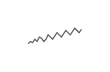
\begin{tikzpicture}[x=0.08em, y=0.08em, line width=0.4pt]
                \draw[FooterGray] (0,3) -- (1,4) -- (2,3.5) -- (3,5) -- (4,4) -- (5,6) -- (6,5.5) -- (7,4) -- (8,5) -- (9,7) -- (10,6) -- (11,5) -- (12,6.5) -- (13,8) -- (14,7) -- (15,6) -- (16,7.5) -- (17,9) -- (18,8) -- (19,7) -- (20,8.5) -- (21,10) -- (22,9) -- (23,8) -- (24,9.5);
            \end{tikzpicture}%
        }%
        \hskip0.5cm%
    }%
    \vskip6pt%
}

%=============================================================================
% PACKAGES
%=============================================================================
\usepackage[utf8]{inputenc}
\DeclareUnicodeCharacter{03B1}{\ensuremath{\alpha}}
\usepackage[T1]{fontenc}
\usepackage{amsmath, amssymb, amsthm}
\usepackage{mathtools}
\usepackage{bm}
\usepackage{tikz}
\usetikzlibrary{arrows.meta, positioning, shapes, calc, decorations.pathreplacing, shadings}
\usepackage{booktabs}
\usepackage{multirow}
\usepackage{array}
\usepackage{graphicx}
\usepackage{animate}
\usepackage{hyperref}
\usepackage{colortbl}
\usepackage{listings}
\lstset{language=Python, basicstyle=\ttfamily\scriptsize, keywordstyle=\color{MainBlue}\bfseries,
  commentstyle=\color{Forest}, stringstyle=\color{Crimson}, breaklines=true,
  frame=none, backgroundcolor=\color{VeryLightGray}, xleftmargin=2mm}
\hypersetup{colorlinks=true, linkcolor=MainBlue, urlcolor=MainBlue}
\graphicspath{{../../logos/}{../../charts/}{../../photos/}}
\usepackage{xcolor}
\hfuzz=2pt  % Suppress tiny overfull warnings (<2pt)
\vfuzz=2pt  % Suppress tiny vertical overfull warnings (<2pt)
% \mathrm in the sans-serif family of the slides (beamer resets \mathrm to the serif family at \begin{document};
% this hook runs after beamer's, so WN, Var, RMSE, ... in formulas match the surrounding text)
% Bold vectors and matrices in the same sans-serif family: \mathbf{A} in sans bold (beamer's own \mathbf came out in
% medium weight), and the bold upright Greek capitals of \boldsymbol / \bm (\bSigma, \bPhi, \boldsymbol{\Theta}) in
% cmss bold: bm.sty fixes its "boldoperators" font when it is loaded (serif cmbx), before beamer switches the
% operators to cmss, so it is reset here.
\AtBeginDocument{%
  \SetMathAlphabet{\mathrm}{normal}{\encodingdefault}{\sfdefault}{\mddefault}{n}%
  \SetMathAlphabet{\mathrm}{bold}{\encodingdefault}{\sfdefault}{bx}{n}%
  \SetMathAlphabet{\mathbf}{normal}{\encodingdefault}{\sfdefault}{bx}{n}%
  \SetMathAlphabet{\mathbf}{bold}{\encodingdefault}{\sfdefault}{bx}{n}%
  \SetSymbolFont{boldoperators}{normal}{OT1}{cmss}{bx}{n}%
  \SetSymbolFont{boldoperators}{bold}{OT1}{cmss}{bx}{n}}

%=============================================================================
% QUANTLET COMMANDS
%   \quantlet{<displayed name>}{<url>}       (generic, compatible with the older TSA decks)
%   \tsaquantlet{Ch_05}{TSA_ch5_garch}       -> https://github.com/danpele/Time-Series-Analysis/tree/main/Quantlets/Ch_05/TSA_ch5_garch
%   \qlurl{<folder>} is defined per chapter by the generator (Quantlets/Ch_NN/<folder>)
%=============================================================================
\newcommand{\tsarepo}{https://github.com/danpele/Time-Series-Analysis}
\newcommand{\tsaqlbase}{https://github.com/danpele/Time-Series-Analysis/tree/main/Quantlets}
\newcommand{\quantlet}[2]{%
    \hfill\href{#2}{%
        \raisebox{-0.15em}{
\includegraphics[height=0.7em]{ql_logo.png}}%
        \textcolor{MainBlue}{\tiny\ #1}%
    }%
}
\newcommand{\tsaquantlet}[2]{\quantlet{\detokenize{#2}}{\tsaqlbase/#1/#2}}

%=============================================================================
% NOTEBOOKS (Google Colab)
%   \colaburl{notebooks/EN/chapter5_seminar_notebook.ipynb} -> the Colab link of a file in the TSA repo
%   \nb: the chapter notebook (each seminar deck redefines it with \renewcommand)
%=============================================================================
\newcommand{\colaburl}[1]{https://colab.research.google.com/github/danpele/Time-Series-Analysis/blob/main/#1}
\newcommand{\nb}{https://colab.research.google.com/github/danpele/Time-Series-Analysis/tree/main/notebooks/EN}
\newcommand{\nbname}{notebooks/EN}

%=============================================================================
% SLIDE HELPERS (used by the generators; the same as in MFM)
%=============================================================================
% local font size for list bodies (the preamble forces \normalsize)
\newcommand{\itemsize}[1]{\setbeamertemplate{itemize/enumerate body begin}{#1}\setbeamertemplate{itemize/enumerate subbody begin}{#1}}
\newcommand{\intitle}[1]{{\hypersetup{urlcolor=white}#1}}   % white links inside coloured title bars
\newcommand{\imgcap}[1]{{\scriptsize #1}\\[0.5mm]}          % caption under a photo
\newcommand{\imgcredit}[2]{{\tiny\color{FooterGray}\href{#1}{#2}}}   % image credit: source URL, author/licence
\newcommand{\aiprompt}[1]{{\ttfamily\color{MainBlue}#1}}     % a prompt to an AI assistant

%=============================================================================
% SEMINARS: student version by default; the instructor wrapper *_solutions.tex sets \solutionstrue
%=============================================================================
\makeatletter\@ifundefined{ifsolutions}{\expandafter\newif\csname ifsolutions\endcsname}{}\makeatother
\newcommand{\solonly}[1]{\ifsolutions #1\fi}
\newcommand{\propsub}{\ifsolutions\else\framesubtitle{\ifdefined\tsalang Rezolvarea se discută la seminar\else Solution discussed in class\fi}\fi}

%=============================================================================
% APPENDIX AND CHAPTER LINKS (latex/appendix_links.py writes the calls; it also re-declares these
% macros before \begin{document}, so the decks compile with or without this preamble block)
%=============================================================================
\providecommand{\tsaapplink}[3]{\hypertarget{#2}{}\hyperlink{#1}{\beamergotobutton{#3}}}
\providecommand{\tsaappback}[2]{\begin{tikzpicture}[remember picture,overlay]\node[anchor=south east] at ([xshift=-3mm,yshift=7mm]current page.south east){\hyperlink{#1}{\beamerreturnbutton{#2}}};\end{tikzpicture}}
\providecommand{\tsachlink}[2]{\href{#1}{#2}}
\providecommand{\tsachlinkt}[2]{\href{#1}{\usebeamercolor[fg]{frametitle}#2}}

%=============================================================================
% QUANTINAR COMMAND: link către un curs Quantinar (subiecte avansate)
%=============================================================================
\newcommand{\quantinar}[2]{%
    \href{#2}{%
        \raisebox{-0.15em}{
\includegraphics[height=0.8em]{qr_logo.png}}%
        \textcolor{MainBlue}{\scriptsize\ #1}%
    }%
}

%=============================================================================
% CUSTOM TITLE PAGE
%=============================================================================
\defbeamertemplate*{title page}{hybrid}[1][]
{
    \vspace{0.2cm}
    % Logos row - top header (with clickable links)
    \begin{center}
        \href{https://www.ase.ro}{
\includegraphics[height=1.0cm]{ase_logo.png}}\hspace{0.3cm}%
        \href{https://theida.net}{
\includegraphics[height=1.0cm]{ida_logo.png}}\hspace{0.3cm}%
        \href{https://blockchain-research-center.com}{
\includegraphics[height=1.0cm]{brc_logo.png}}\hspace{0.3cm}%
        \href{https://www.ai4efin.ase.ro}{
\includegraphics[height=1.0cm]{ai4efin_logo.png}}\hspace{0.3cm}%
        \href{https://ipe.ro/new}{
\includegraphics[height=1.0cm]{acad_logo.png}}\hspace{0.3cm}%
        \href{https://www.digital-finance-msca.com}{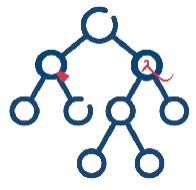
\includegraphics[height=1.0cm]{msca_logo.png}}%
    \end{center}

    \vspace{0.6cm}

    % Main title with Q logos on sides (with clickable links)
    \begin{center}
        \begin{minipage}{0.1\textwidth}
            \centering
            \href{https://quantlet.com}{
\includegraphics[height=1.1cm]{ql_logo.png}}
        \end{minipage}%
        \begin{minipage}{0.78\textwidth}
            \centering
            {\LARGE\bfseries\usebeamercolor[fg]{title}\inserttitle}

            \vspace{0.3cm}

            {\usebeamerfont{subtitle}\usebeamercolor[fg]{title}\insertsubtitle}
        \end{minipage}%
        \begin{minipage}{0.1\textwidth}
            \centering
            \href{https://quantinar.com}{
\includegraphics[height=1.1cm]{qr_logo.png}}
        \end{minipage}
    \end{center}

    \vspace{0.6cm}

    % Authors (left aligned)
    \hspace{0.5cm}{\usebeamerfont{author}\insertauthor}

    \vspace{0.3cm}

    % Institute/Affiliations (left aligned)
    \hspace{0.5cm}\begin{minipage}[t]{0.9\textwidth}
        \raggedright\small\insertinstitute
    \end{minipage}
}

%=============================================================================
% THEOREM ENVIRONMENTS
%=============================================================================
\theoremstyle{definition}
\setbeamertemplate{theorems}[numbered]
\ifdefined\tsalang
\newtheorem{defn}{Definiție}
\newtheorem{thm}{Teoremă}
\newtheorem{prop}{Propoziție}
\newtheorem{rmk}{Observație}
\else
\newtheorem{defn}{Definition}
\newtheorem{thm}{Theorem}
\newtheorem{prop}{Proposition}
\newtheorem{rmk}{Remark}
\fi

%=============================================================================
% CENTRED MINIPAGE (no extra vertical space)
%=============================================================================
\newenvironment{cminipage}[1]{%
    \par\noindent\hfill\begin{minipage}{#1}\ignorespaces
}{%
    \end{minipage}\hfill\null\par
}

%=============================================================================
% CUSTOM COMMANDS
%=============================================================================
\newcommand{\E}{\mathbb{E}}
\newcommand{\Var}{\text{Var}}
\newcommand{\Cov}{\text{Cov}}
\newcommand{\Corr}{\text{Corr}}
\newcommand{\R}{\mathbb{R}}
\newcommand{\N}{\mathbb{N}}
\newcommand{\Z}{\mathbb{Z}}
\newcommand{\B}{\mathbf{B}}
\newcommand{\imark}{\textcolor{MainBlue}{\textbullet}}
\newcommand{\RMSE}{\text{RMSE}}
\newcommand{\MAE}{\text{MAE}}
\newcommand{\MAPE}{\text{MAPE}}

% Boldface vector/matrix commands (VAR, VECM, state space; also used by the older TSA decks)
\newcommand{\bY}{\mathbf{Y}}
\newcommand{\bX}{\mathbf{X}}
\newcommand{\bA}{\mathbf{A}}
\newcommand{\bB}{\mathbf{B}}
\newcommand{\bepsilon}{\boldsymbol{\varepsilon}}
\newcommand{\bSigma}{\boldsymbol{\Sigma}}
\newcommand{\bPhi}{\boldsymbol{\Phi}}
\newcommand{\bGamma}{\boldsymbol{\Gamma}}
\newcommand{\bPi}{\boldsymbol{\Pi}}
\newcommand{\bc}{\mathbf{c}}
\newcommand{\balpha}{\boldsymbol{\alpha}}
\newcommand{\bbeta}{\boldsymbol{\beta}}
\newcommand{\bvarepsilon}{\boldsymbol{\varepsilon}}

% Legacy seminar marks (older TSA seminar decks)
\newcommand{\correct}{\textcolor{Forest}{\checkmark}}
\newcommand{\incorrect}{\textcolor{Crimson}{\texttimes}}
 se definește
%   \newcommand{\coursename}{Time Series Analysis}      (EN)
%   \newcommand{\coursename}{Serii de timp}       (RO)  și  \def\tsalang{ro}
% Fișierele .tex se află în EN/Courses, EN/Seminars, RO/Cursuri, RO/Seminarii (două niveluri sub rădăcină).
% Deck-urile sînt generate de latex/build_chapterN.py / build_seminarN.py (vezi latex/tsa_build.py).

\documentclass[9pt, aspectratio=169, t]{beamer}
\providecommand{\coursename}{Time Series Analysis}

% Ensure content fits on slides
\setbeamersize{text margin left=8mm, text margin right=8mm}
% Smaller institute font (title page)
\setbeamerfont{institute}{size=\footnotesize}

%=============================================================================
% THEME AND STYLE CONFIGURATION
%=============================================================================
\usetheme{default}
% Using default theme for clean header/footer control

% Color Palette (matching Redispatch PDF)
\definecolor{MainBlue}{RGB}{26, 58, 110}
\definecolor{AccentBlue}{RGB}{26, 58, 110}
\definecolor{IDAred}{RGB}{205, 0, 0}
\definecolor{DarkGray}{RGB}{51, 51, 51}
\definecolor{MediumGray}{RGB}{128, 128, 128}
\definecolor{LightGray}{RGB}{248, 248, 248}
\definecolor{VeryLightGray}{RGB}{235, 235, 235}
\definecolor{KeynoteGray}{RGB}{218, 218, 218}
\definecolor{SectionGray}{RGB}{120, 120, 120}
\definecolor{FooterGray}{RGB}{100, 100, 100}
\definecolor{Crimson}{RGB}{220, 53, 69}
\definecolor{Forest}{RGB}{46, 125, 50}
\definecolor{Amber}{RGB}{181, 133, 63}
\definecolor{Orange}{RGB}{230, 126, 34}
\definecolor{Purple}{RGB}{142, 68, 173}

% Gradient background (exact Keynote 315° gradient: white to RGB 218,218,218)
\setbeamertemplate{background}{%
    \begin{tikzpicture}[remember picture, overlay]
        \shade[shading=axis, shading angle=315,
        top color=white, bottom color=KeynoteGray]
        (current page.south west) rectangle (current page.north east);
    \end{tikzpicture}%
}
% Fallback solid color for compatibility
\setbeamercolor{background canvas}{bg=}

\setbeamercolor{palette primary}{bg=MainBlue, fg=white}
\setbeamercolor{palette secondary}{bg=MainBlue!85, fg=white}
\setbeamercolor{palette tertiary}{bg=MainBlue!70, fg=white}
\setbeamercolor{structure}{fg=MainBlue}
\setbeamercolor{title}{fg=IDAred}
\setbeamercolor{frametitle}{fg=IDAred, bg=}
\setbeamercolor{block title}{bg=MainBlue, fg=white}
\setbeamercolor{block body}{bg=VeryLightGray, fg=DarkGray}
\setbeamercolor{block title alerted}{bg=Crimson, fg=white}
\setbeamercolor{block body alerted}{bg=Crimson!8, fg=DarkGray}
\setbeamercolor{block title example}{bg=Forest, fg=white}
\setbeamercolor{block body example}{bg=Forest!8, fg=DarkGray}
\setbeamercolor{item}{fg=MainBlue}

% Footer colors (override Madrid theme blue)
\setbeamercolor{author in head/foot}{fg=FooterGray, bg=}
\setbeamercolor{title in head/foot}{fg=FooterGray, bg=}
\setbeamercolor{date in head/foot}{fg=FooterGray, bg=}
\setbeamercolor{section in head/foot}{fg=FooterGray, bg=}
\setbeamercolor{subsection in head/foot}{fg=FooterGray, bg=}

% Bullet styles (apply everywhere including blocks)
\setbeamertemplate{itemize item}{\color{MainBlue}$\boxdot$}
\setbeamertemplate{itemize subitem}{\color{MainBlue}$\blacktriangleright$}
\setbeamertemplate{itemize subsubitem}{\color{MainBlue}\tiny$\bullet$}
\setbeamertemplate{itemize/enumerate body begin}{\normalsize}
\setbeamertemplate{itemize/enumerate subbody begin}{\normalsize}

% Item spacing - compact style
\setlength{\leftmargini}{10pt}       % Level 1: minimal indent
\setlength{\leftmarginii}{10pt}      % Level 2: minimal additional indent
% Compact list spacing (zero extra space before/after lists in blocks)
\makeatletter
\def\@listi{\leftmargin\leftmargini \topsep 0pt \parsep 0pt \itemsep 0pt}
\def\@listii{\leftmargin\leftmarginii \topsep 0pt \parsep 0pt \itemsep 0pt}
\makeatother

\setbeamertemplate{navigation symbols}{}

%=============================================================================
% CUSTOM HEADLINE
%=============================================================================
\setbeamertemplate{headline}{%
    \vskip10pt%
    \hbox to \paperwidth{%
        \hskip0.5cm%
        {\small\color{FooterGray}\renewcommand{\hyperlink}[2]{##2}\insertsectionhead}%
        \hfill%
        \textcolor{FooterGray}{\small\insertframenumber}%
        \hskip0.5cm%
    }%
    \vskip4pt%
    {\color{FooterGray}\hrule height 0.4pt}%
}

%=============================================================================
% CUSTOM FOOTER
%=============================================================================
\usepackage{fontawesome5}

\setbeamertemplate{footline}{%
    {\color{FooterGray}\hrule height 0.4pt}%
    \vskip4pt%
    \hbox to \paperwidth{%
        \hskip0.5cm%
        \textcolor{FooterGray}{\small\coursename}%
        \hfill%
        \raisebox{-0.1em}{%
            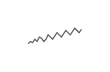
\begin{tikzpicture}[x=0.08em, y=0.08em, line width=0.4pt]
                \draw[FooterGray] (0,3) -- (1,4) -- (2,3.5) -- (3,5) -- (4,4) -- (5,6) -- (6,5.5) -- (7,4) -- (8,5) -- (9,7) -- (10,6) -- (11,5) -- (12,6.5) -- (13,8) -- (14,7) -- (15,6) -- (16,7.5) -- (17,9) -- (18,8) -- (19,7) -- (20,8.5) -- (21,10) -- (22,9) -- (23,8) -- (24,9.5);
            \end{tikzpicture}%
        }%
        \hskip0.5cm%
    }%
    \vskip6pt%
}

%=============================================================================
% PACKAGES
%=============================================================================
\usepackage[utf8]{inputenc}
\DeclareUnicodeCharacter{03B1}{\ensuremath{\alpha}}
\usepackage[T1]{fontenc}
\usepackage{amsmath, amssymb, amsthm}
\usepackage{mathtools}
\usepackage{bm}
\usepackage{tikz}
\usetikzlibrary{arrows.meta, positioning, shapes, calc, decorations.pathreplacing, shadings}
\usepackage{booktabs}
\usepackage{multirow}
\usepackage{array}
\usepackage{graphicx}
\usepackage{animate}
\usepackage{hyperref}
\usepackage{colortbl}
\usepackage{listings}
\lstset{language=Python, basicstyle=\ttfamily\scriptsize, keywordstyle=\color{MainBlue}\bfseries,
  commentstyle=\color{Forest}, stringstyle=\color{Crimson}, breaklines=true,
  frame=none, backgroundcolor=\color{VeryLightGray}, xleftmargin=2mm}
\hypersetup{colorlinks=true, linkcolor=MainBlue, urlcolor=MainBlue}
\graphicspath{{../../logos/}{../../charts/}{../../photos/}}
\usepackage{xcolor}
\hfuzz=2pt  % Suppress tiny overfull warnings (<2pt)
\vfuzz=2pt  % Suppress tiny vertical overfull warnings (<2pt)
% \mathrm in the sans-serif family of the slides (beamer resets \mathrm to the serif family at \begin{document};
% this hook runs after beamer's, so WN, Var, RMSE, ... in formulas match the surrounding text)
% Bold vectors and matrices in the same sans-serif family: \mathbf{A} in sans bold (beamer's own \mathbf came out in
% medium weight), and the bold upright Greek capitals of \boldsymbol / \bm (\bSigma, \bPhi, \boldsymbol{\Theta}) in
% cmss bold: bm.sty fixes its "boldoperators" font when it is loaded (serif cmbx), before beamer switches the
% operators to cmss, so it is reset here.
\AtBeginDocument{%
  \SetMathAlphabet{\mathrm}{normal}{\encodingdefault}{\sfdefault}{\mddefault}{n}%
  \SetMathAlphabet{\mathrm}{bold}{\encodingdefault}{\sfdefault}{bx}{n}%
  \SetMathAlphabet{\mathbf}{normal}{\encodingdefault}{\sfdefault}{bx}{n}%
  \SetMathAlphabet{\mathbf}{bold}{\encodingdefault}{\sfdefault}{bx}{n}%
  \SetSymbolFont{boldoperators}{normal}{OT1}{cmss}{bx}{n}%
  \SetSymbolFont{boldoperators}{bold}{OT1}{cmss}{bx}{n}}

%=============================================================================
% QUANTLET COMMANDS
%   \quantlet{<displayed name>}{<url>}       (generic, compatible with the older TSA decks)
%   \tsaquantlet{Ch_05}{TSA_ch5_garch}       -> https://github.com/danpele/Time-Series-Analysis/tree/main/Quantlets/Ch_05/TSA_ch5_garch
%   \qlurl{<folder>} is defined per chapter by the generator (Quantlets/Ch_NN/<folder>)
%=============================================================================
\newcommand{\tsarepo}{https://github.com/danpele/Time-Series-Analysis}
\newcommand{\tsaqlbase}{https://github.com/danpele/Time-Series-Analysis/tree/main/Quantlets}
\newcommand{\quantlet}[2]{%
    \hfill\href{#2}{%
        \raisebox{-0.15em}{
\includegraphics[height=0.7em]{ql_logo.png}}%
        \textcolor{MainBlue}{\tiny\ #1}%
    }%
}
\newcommand{\tsaquantlet}[2]{\quantlet{\detokenize{#2}}{\tsaqlbase/#1/#2}}

%=============================================================================
% NOTEBOOKS (Google Colab)
%   \colaburl{notebooks/EN/chapter5_seminar_notebook.ipynb} -> the Colab link of a file in the TSA repo
%   \nb: the chapter notebook (each seminar deck redefines it with \renewcommand)
%=============================================================================
\newcommand{\colaburl}[1]{https://colab.research.google.com/github/danpele/Time-Series-Analysis/blob/main/#1}
\newcommand{\nb}{https://colab.research.google.com/github/danpele/Time-Series-Analysis/tree/main/notebooks/EN}
\newcommand{\nbname}{notebooks/EN}

%=============================================================================
% SLIDE HELPERS (used by the generators; the same as in MFM)
%=============================================================================
% local font size for list bodies (the preamble forces \normalsize)
\newcommand{\itemsize}[1]{\setbeamertemplate{itemize/enumerate body begin}{#1}\setbeamertemplate{itemize/enumerate subbody begin}{#1}}
\newcommand{\intitle}[1]{{\hypersetup{urlcolor=white}#1}}   % white links inside coloured title bars
\newcommand{\imgcap}[1]{{\scriptsize #1}\\[0.5mm]}          % caption under a photo
\newcommand{\imgcredit}[2]{{\tiny\color{FooterGray}\href{#1}{#2}}}   % image credit: source URL, author/licence
\newcommand{\aiprompt}[1]{{\ttfamily\color{MainBlue}#1}}     % a prompt to an AI assistant

%=============================================================================
% SEMINARS: student version by default; the instructor wrapper *_solutions.tex sets \solutionstrue
%=============================================================================
\makeatletter\@ifundefined{ifsolutions}{\expandafter\newif\csname ifsolutions\endcsname}{}\makeatother
\newcommand{\solonly}[1]{\ifsolutions #1\fi}
\newcommand{\propsub}{\ifsolutions\else\framesubtitle{\ifdefined\tsalang Rezolvarea se discută la seminar\else Solution discussed in class\fi}\fi}

%=============================================================================
% APPENDIX AND CHAPTER LINKS (latex/appendix_links.py writes the calls; it also re-declares these
% macros before \begin{document}, so the decks compile with or without this preamble block)
%=============================================================================
\providecommand{\tsaapplink}[3]{\hypertarget{#2}{}\hyperlink{#1}{\beamergotobutton{#3}}}
\providecommand{\tsaappback}[2]{\begin{tikzpicture}[remember picture,overlay]\node[anchor=south east] at ([xshift=-3mm,yshift=7mm]current page.south east){\hyperlink{#1}{\beamerreturnbutton{#2}}};\end{tikzpicture}}
\providecommand{\tsachlink}[2]{\href{#1}{#2}}
\providecommand{\tsachlinkt}[2]{\href{#1}{\usebeamercolor[fg]{frametitle}#2}}

%=============================================================================
% QUANTINAR COMMAND: link către un curs Quantinar (subiecte avansate)
%=============================================================================
\newcommand{\quantinar}[2]{%
    \href{#2}{%
        \raisebox{-0.15em}{
\includegraphics[height=0.8em]{qr_logo.png}}%
        \textcolor{MainBlue}{\scriptsize\ #1}%
    }%
}

%=============================================================================
% CUSTOM TITLE PAGE
%=============================================================================
\defbeamertemplate*{title page}{hybrid}[1][]
{
    \vspace{0.2cm}
    % Logos row - top header (with clickable links)
    \begin{center}
        \href{https://www.ase.ro}{
\includegraphics[height=1.0cm]{ase_logo.png}}\hspace{0.3cm}%
        \href{https://theida.net}{
\includegraphics[height=1.0cm]{ida_logo.png}}\hspace{0.3cm}%
        \href{https://blockchain-research-center.com}{
\includegraphics[height=1.0cm]{brc_logo.png}}\hspace{0.3cm}%
        \href{https://www.ai4efin.ase.ro}{
\includegraphics[height=1.0cm]{ai4efin_logo.png}}\hspace{0.3cm}%
        \href{https://ipe.ro/new}{
\includegraphics[height=1.0cm]{acad_logo.png}}\hspace{0.3cm}%
        \href{https://www.digital-finance-msca.com}{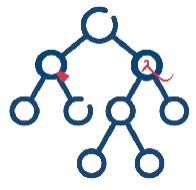
\includegraphics[height=1.0cm]{msca_logo.png}}%
    \end{center}

    \vspace{0.6cm}

    % Main title with Q logos on sides (with clickable links)
    \begin{center}
        \begin{minipage}{0.1\textwidth}
            \centering
            \href{https://quantlet.com}{
\includegraphics[height=1.1cm]{ql_logo.png}}
        \end{minipage}%
        \begin{minipage}{0.78\textwidth}
            \centering
            {\LARGE\bfseries\usebeamercolor[fg]{title}\inserttitle}

            \vspace{0.3cm}

            {\usebeamerfont{subtitle}\usebeamercolor[fg]{title}\insertsubtitle}
        \end{minipage}%
        \begin{minipage}{0.1\textwidth}
            \centering
            \href{https://quantinar.com}{
\includegraphics[height=1.1cm]{qr_logo.png}}
        \end{minipage}
    \end{center}

    \vspace{0.6cm}

    % Authors (left aligned)
    \hspace{0.5cm}{\usebeamerfont{author}\insertauthor}

    \vspace{0.3cm}

    % Institute/Affiliations (left aligned)
    \hspace{0.5cm}\begin{minipage}[t]{0.9\textwidth}
        \raggedright\small\insertinstitute
    \end{minipage}
}

%=============================================================================
% THEOREM ENVIRONMENTS
%=============================================================================
\theoremstyle{definition}
\setbeamertemplate{theorems}[numbered]
\ifdefined\tsalang
\newtheorem{defn}{Definiție}
\newtheorem{thm}{Teoremă}
\newtheorem{prop}{Propoziție}
\newtheorem{rmk}{Observație}
\else
\newtheorem{defn}{Definition}
\newtheorem{thm}{Theorem}
\newtheorem{prop}{Proposition}
\newtheorem{rmk}{Remark}
\fi

%=============================================================================
% CENTRED MINIPAGE (no extra vertical space)
%=============================================================================
\newenvironment{cminipage}[1]{%
    \par\noindent\hfill\begin{minipage}{#1}\ignorespaces
}{%
    \end{minipage}\hfill\null\par
}

%=============================================================================
% CUSTOM COMMANDS
%=============================================================================
\newcommand{\E}{\mathbb{E}}
\newcommand{\Var}{\text{Var}}
\newcommand{\Cov}{\text{Cov}}
\newcommand{\Corr}{\text{Corr}}
\newcommand{\R}{\mathbb{R}}
\newcommand{\N}{\mathbb{N}}
\newcommand{\Z}{\mathbb{Z}}
\newcommand{\B}{\mathbf{B}}
\newcommand{\imark}{\textcolor{MainBlue}{\textbullet}}
\newcommand{\RMSE}{\text{RMSE}}
\newcommand{\MAE}{\text{MAE}}
\newcommand{\MAPE}{\text{MAPE}}

% Boldface vector/matrix commands (VAR, VECM, state space; also used by the older TSA decks)
\newcommand{\bY}{\mathbf{Y}}
\newcommand{\bX}{\mathbf{X}}
\newcommand{\bA}{\mathbf{A}}
\newcommand{\bB}{\mathbf{B}}
\newcommand{\bepsilon}{\boldsymbol{\varepsilon}}
\newcommand{\bSigma}{\boldsymbol{\Sigma}}
\newcommand{\bPhi}{\boldsymbol{\Phi}}
\newcommand{\bGamma}{\boldsymbol{\Gamma}}
\newcommand{\bPi}{\boldsymbol{\Pi}}
\newcommand{\bc}{\mathbf{c}}
\newcommand{\balpha}{\boldsymbol{\alpha}}
\newcommand{\bbeta}{\boldsymbol{\beta}}
\newcommand{\bvarepsilon}{\boldsymbol{\varepsilon}}

% Legacy seminar marks (older TSA seminar decks)
\newcommand{\correct}{\textcolor{Forest}{\checkmark}}
\newcommand{\incorrect}{\textcolor{Crimson}{\texttimes}}
 se definește
%   \newcommand{\coursename}{Time Series Analysis}      (EN)
%   \newcommand{\coursename}{Serii de timp}       (RO)  și  \def\tsalang{ro}
% Fișierele .tex se află în EN/Courses, EN/Seminars, RO/Cursuri, RO/Seminarii (două niveluri sub rădăcină).
% Deck-urile sînt generate de latex/build_chapterN.py / build_seminarN.py (vezi latex/tsa_build.py).

\documentclass[9pt, aspectratio=169, t]{beamer}
\providecommand{\coursename}{Time Series Analysis}

% Ensure content fits on slides
\setbeamersize{text margin left=8mm, text margin right=8mm}
% Smaller institute font (title page)
\setbeamerfont{institute}{size=\footnotesize}

%=============================================================================
% THEME AND STYLE CONFIGURATION
%=============================================================================
\usetheme{default}
% Using default theme for clean header/footer control

% Color Palette (matching Redispatch PDF)
\definecolor{MainBlue}{RGB}{26, 58, 110}
\definecolor{AccentBlue}{RGB}{26, 58, 110}
\definecolor{IDAred}{RGB}{205, 0, 0}
\definecolor{DarkGray}{RGB}{51, 51, 51}
\definecolor{MediumGray}{RGB}{128, 128, 128}
\definecolor{LightGray}{RGB}{248, 248, 248}
\definecolor{VeryLightGray}{RGB}{235, 235, 235}
\definecolor{KeynoteGray}{RGB}{218, 218, 218}
\definecolor{SectionGray}{RGB}{120, 120, 120}
\definecolor{FooterGray}{RGB}{100, 100, 100}
\definecolor{Crimson}{RGB}{220, 53, 69}
\definecolor{Forest}{RGB}{46, 125, 50}
\definecolor{Amber}{RGB}{181, 133, 63}
\definecolor{Orange}{RGB}{230, 126, 34}
\definecolor{Purple}{RGB}{142, 68, 173}

% Gradient background (exact Keynote 315° gradient: white to RGB 218,218,218)
\setbeamertemplate{background}{%
    \begin{tikzpicture}[remember picture, overlay]
        \shade[shading=axis, shading angle=315,
        top color=white, bottom color=KeynoteGray]
        (current page.south west) rectangle (current page.north east);
    \end{tikzpicture}%
}
% Fallback solid color for compatibility
\setbeamercolor{background canvas}{bg=}

\setbeamercolor{palette primary}{bg=MainBlue, fg=white}
\setbeamercolor{palette secondary}{bg=MainBlue!85, fg=white}
\setbeamercolor{palette tertiary}{bg=MainBlue!70, fg=white}
\setbeamercolor{structure}{fg=MainBlue}
\setbeamercolor{title}{fg=IDAred}
\setbeamercolor{frametitle}{fg=IDAred, bg=}
\setbeamercolor{block title}{bg=MainBlue, fg=white}
\setbeamercolor{block body}{bg=VeryLightGray, fg=DarkGray}
\setbeamercolor{block title alerted}{bg=Crimson, fg=white}
\setbeamercolor{block body alerted}{bg=Crimson!8, fg=DarkGray}
\setbeamercolor{block title example}{bg=Forest, fg=white}
\setbeamercolor{block body example}{bg=Forest!8, fg=DarkGray}
\setbeamercolor{item}{fg=MainBlue}

% Footer colors (override Madrid theme blue)
\setbeamercolor{author in head/foot}{fg=FooterGray, bg=}
\setbeamercolor{title in head/foot}{fg=FooterGray, bg=}
\setbeamercolor{date in head/foot}{fg=FooterGray, bg=}
\setbeamercolor{section in head/foot}{fg=FooterGray, bg=}
\setbeamercolor{subsection in head/foot}{fg=FooterGray, bg=}

% Bullet styles (apply everywhere including blocks)
\setbeamertemplate{itemize item}{\color{MainBlue}$\boxdot$}
\setbeamertemplate{itemize subitem}{\color{MainBlue}$\blacktriangleright$}
\setbeamertemplate{itemize subsubitem}{\color{MainBlue}\tiny$\bullet$}
\setbeamertemplate{itemize/enumerate body begin}{\normalsize}
\setbeamertemplate{itemize/enumerate subbody begin}{\normalsize}

% Item spacing - compact style
\setlength{\leftmargini}{10pt}       % Level 1: minimal indent
\setlength{\leftmarginii}{10pt}      % Level 2: minimal additional indent
% Compact list spacing (zero extra space before/after lists in blocks)
\makeatletter
\def\@listi{\leftmargin\leftmargini \topsep 0pt \parsep 0pt \itemsep 0pt}
\def\@listii{\leftmargin\leftmarginii \topsep 0pt \parsep 0pt \itemsep 0pt}
\makeatother

\setbeamertemplate{navigation symbols}{}

%=============================================================================
% CUSTOM HEADLINE
%=============================================================================
\setbeamertemplate{headline}{%
    \vskip10pt%
    \hbox to \paperwidth{%
        \hskip0.5cm%
        {\small\color{FooterGray}\renewcommand{\hyperlink}[2]{##2}\insertsectionhead}%
        \hfill%
        \textcolor{FooterGray}{\small\insertframenumber}%
        \hskip0.5cm%
    }%
    \vskip4pt%
    {\color{FooterGray}\hrule height 0.4pt}%
}

%=============================================================================
% CUSTOM FOOTER
%=============================================================================
\usepackage{fontawesome5}

\setbeamertemplate{footline}{%
    {\color{FooterGray}\hrule height 0.4pt}%
    \vskip4pt%
    \hbox to \paperwidth{%
        \hskip0.5cm%
        \textcolor{FooterGray}{\small\coursename}%
        \hfill%
        \raisebox{-0.1em}{%
            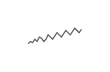
\begin{tikzpicture}[x=0.08em, y=0.08em, line width=0.4pt]
                \draw[FooterGray] (0,3) -- (1,4) -- (2,3.5) -- (3,5) -- (4,4) -- (5,6) -- (6,5.5) -- (7,4) -- (8,5) -- (9,7) -- (10,6) -- (11,5) -- (12,6.5) -- (13,8) -- (14,7) -- (15,6) -- (16,7.5) -- (17,9) -- (18,8) -- (19,7) -- (20,8.5) -- (21,10) -- (22,9) -- (23,8) -- (24,9.5);
            \end{tikzpicture}%
        }%
        \hskip0.5cm%
    }%
    \vskip6pt%
}

%=============================================================================
% PACKAGES
%=============================================================================
\usepackage[utf8]{inputenc}
\DeclareUnicodeCharacter{03B1}{\ensuremath{\alpha}}
\usepackage[T1]{fontenc}
\usepackage{amsmath, amssymb, amsthm}
\usepackage{mathtools}
\usepackage{bm}
\usepackage{tikz}
\usetikzlibrary{arrows.meta, positioning, shapes, calc, decorations.pathreplacing, shadings}
\usepackage{booktabs}
\usepackage{multirow}
\usepackage{array}
\usepackage{graphicx}
\usepackage{animate}
\usepackage{hyperref}
\usepackage{colortbl}
\usepackage{listings}
\lstset{language=Python, basicstyle=\ttfamily\scriptsize, keywordstyle=\color{MainBlue}\bfseries,
  commentstyle=\color{Forest}, stringstyle=\color{Crimson}, breaklines=true,
  frame=none, backgroundcolor=\color{VeryLightGray}, xleftmargin=2mm}
\hypersetup{colorlinks=true, linkcolor=MainBlue, urlcolor=MainBlue}
\graphicspath{{../../logos/}{../../charts/}{../../photos/}}
\usepackage{xcolor}
\hfuzz=2pt  % Suppress tiny overfull warnings (<2pt)
\vfuzz=2pt  % Suppress tiny vertical overfull warnings (<2pt)
% \mathrm in the sans-serif family of the slides (beamer resets \mathrm to the serif family at \begin{document};
% this hook runs after beamer's, so WN, Var, RMSE, ... in formulas match the surrounding text)
% Bold vectors and matrices in the same sans-serif family: \mathbf{A} in sans bold (beamer's own \mathbf came out in
% medium weight), and the bold upright Greek capitals of \boldsymbol / \bm (\bSigma, \bPhi, \boldsymbol{\Theta}) in
% cmss bold: bm.sty fixes its "boldoperators" font when it is loaded (serif cmbx), before beamer switches the
% operators to cmss, so it is reset here.
\AtBeginDocument{%
  \SetMathAlphabet{\mathrm}{normal}{\encodingdefault}{\sfdefault}{\mddefault}{n}%
  \SetMathAlphabet{\mathrm}{bold}{\encodingdefault}{\sfdefault}{bx}{n}%
  \SetMathAlphabet{\mathbf}{normal}{\encodingdefault}{\sfdefault}{bx}{n}%
  \SetMathAlphabet{\mathbf}{bold}{\encodingdefault}{\sfdefault}{bx}{n}%
  \SetSymbolFont{boldoperators}{normal}{OT1}{cmss}{bx}{n}%
  \SetSymbolFont{boldoperators}{bold}{OT1}{cmss}{bx}{n}}

%=============================================================================
% QUANTLET COMMANDS
%   \quantlet{<displayed name>}{<url>}       (generic, compatible with the older TSA decks)
%   \tsaquantlet{Ch_05}{TSA_ch5_garch}       -> https://github.com/danpele/Time-Series-Analysis/tree/main/Quantlets/Ch_05/TSA_ch5_garch
%   \qlurl{<folder>} is defined per chapter by the generator (Quantlets/Ch_NN/<folder>)
%=============================================================================
\newcommand{\tsarepo}{https://github.com/danpele/Time-Series-Analysis}
\newcommand{\tsaqlbase}{https://github.com/danpele/Time-Series-Analysis/tree/main/Quantlets}
\newcommand{\quantlet}[2]{%
    \hfill\href{#2}{%
        \raisebox{-0.15em}{
\includegraphics[height=0.7em]{ql_logo.png}}%
        \textcolor{MainBlue}{\tiny\ #1}%
    }%
}
\newcommand{\tsaquantlet}[2]{\quantlet{\detokenize{#2}}{\tsaqlbase/#1/#2}}

%=============================================================================
% NOTEBOOKS (Google Colab)
%   \colaburl{notebooks/EN/chapter5_seminar_notebook.ipynb} -> the Colab link of a file in the TSA repo
%   \nb: the chapter notebook (each seminar deck redefines it with \renewcommand)
%=============================================================================
\newcommand{\colaburl}[1]{https://colab.research.google.com/github/danpele/Time-Series-Analysis/blob/main/#1}
\newcommand{\nb}{https://colab.research.google.com/github/danpele/Time-Series-Analysis/tree/main/notebooks/EN}
\newcommand{\nbname}{notebooks/EN}

%=============================================================================
% SLIDE HELPERS (used by the generators; the same as in MFM)
%=============================================================================
% local font size for list bodies (the preamble forces \normalsize)
\newcommand{\itemsize}[1]{\setbeamertemplate{itemize/enumerate body begin}{#1}\setbeamertemplate{itemize/enumerate subbody begin}{#1}}
\newcommand{\intitle}[1]{{\hypersetup{urlcolor=white}#1}}   % white links inside coloured title bars
\newcommand{\imgcap}[1]{{\scriptsize #1}\\[0.5mm]}          % caption under a photo
\newcommand{\imgcredit}[2]{{\tiny\color{FooterGray}\href{#1}{#2}}}   % image credit: source URL, author/licence
\newcommand{\aiprompt}[1]{{\ttfamily\color{MainBlue}#1}}     % a prompt to an AI assistant

%=============================================================================
% SEMINARS: student version by default; the instructor wrapper *_solutions.tex sets \solutionstrue
%=============================================================================
\makeatletter\@ifundefined{ifsolutions}{\expandafter\newif\csname ifsolutions\endcsname}{}\makeatother
\newcommand{\solonly}[1]{\ifsolutions #1\fi}
\newcommand{\propsub}{\ifsolutions\else\framesubtitle{\ifdefined\tsalang Rezolvarea se discută la seminar\else Solution discussed in class\fi}\fi}

%=============================================================================
% APPENDIX AND CHAPTER LINKS (latex/appendix_links.py writes the calls; it also re-declares these
% macros before \begin{document}, so the decks compile with or without this preamble block)
%=============================================================================
\providecommand{\tsaapplink}[3]{\hypertarget{#2}{}\hyperlink{#1}{\beamergotobutton{#3}}}
\providecommand{\tsaappback}[2]{\begin{tikzpicture}[remember picture,overlay]\node[anchor=south east] at ([xshift=-3mm,yshift=7mm]current page.south east){\hyperlink{#1}{\beamerreturnbutton{#2}}};\end{tikzpicture}}
\providecommand{\tsachlink}[2]{\href{#1}{#2}}
\providecommand{\tsachlinkt}[2]{\href{#1}{\usebeamercolor[fg]{frametitle}#2}}

%=============================================================================
% QUANTINAR COMMAND: link către un curs Quantinar (subiecte avansate)
%=============================================================================
\newcommand{\quantinar}[2]{%
    \href{#2}{%
        \raisebox{-0.15em}{
\includegraphics[height=0.8em]{qr_logo.png}}%
        \textcolor{MainBlue}{\scriptsize\ #1}%
    }%
}

%=============================================================================
% CUSTOM TITLE PAGE
%=============================================================================
\defbeamertemplate*{title page}{hybrid}[1][]
{
    \vspace{0.2cm}
    % Logos row - top header (with clickable links)
    \begin{center}
        \href{https://www.ase.ro}{
\includegraphics[height=1.0cm]{ase_logo.png}}\hspace{0.3cm}%
        \href{https://theida.net}{
\includegraphics[height=1.0cm]{ida_logo.png}}\hspace{0.3cm}%
        \href{https://blockchain-research-center.com}{
\includegraphics[height=1.0cm]{brc_logo.png}}\hspace{0.3cm}%
        \href{https://www.ai4efin.ase.ro}{
\includegraphics[height=1.0cm]{ai4efin_logo.png}}\hspace{0.3cm}%
        \href{https://ipe.ro/new}{
\includegraphics[height=1.0cm]{acad_logo.png}}\hspace{0.3cm}%
        \href{https://www.digital-finance-msca.com}{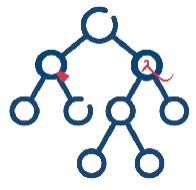
\includegraphics[height=1.0cm]{msca_logo.png}}%
    \end{center}

    \vspace{0.6cm}

    % Main title with Q logos on sides (with clickable links)
    \begin{center}
        \begin{minipage}{0.1\textwidth}
            \centering
            \href{https://quantlet.com}{
\includegraphics[height=1.1cm]{ql_logo.png}}
        \end{minipage}%
        \begin{minipage}{0.78\textwidth}
            \centering
            {\LARGE\bfseries\usebeamercolor[fg]{title}\inserttitle}

            \vspace{0.3cm}

            {\usebeamerfont{subtitle}\usebeamercolor[fg]{title}\insertsubtitle}
        \end{minipage}%
        \begin{minipage}{0.1\textwidth}
            \centering
            \href{https://quantinar.com}{
\includegraphics[height=1.1cm]{qr_logo.png}}
        \end{minipage}
    \end{center}

    \vspace{0.6cm}

    % Authors (left aligned)
    \hspace{0.5cm}{\usebeamerfont{author}\insertauthor}

    \vspace{0.3cm}

    % Institute/Affiliations (left aligned)
    \hspace{0.5cm}\begin{minipage}[t]{0.9\textwidth}
        \raggedright\small\insertinstitute
    \end{minipage}
}

%=============================================================================
% THEOREM ENVIRONMENTS
%=============================================================================
\theoremstyle{definition}
\setbeamertemplate{theorems}[numbered]
\ifdefined\tsalang
\newtheorem{defn}{Definiție}
\newtheorem{thm}{Teoremă}
\newtheorem{prop}{Propoziție}
\newtheorem{rmk}{Observație}
\else
\newtheorem{defn}{Definition}
\newtheorem{thm}{Theorem}
\newtheorem{prop}{Proposition}
\newtheorem{rmk}{Remark}
\fi

%=============================================================================
% CENTRED MINIPAGE (no extra vertical space)
%=============================================================================
\newenvironment{cminipage}[1]{%
    \par\noindent\hfill\begin{minipage}{#1}\ignorespaces
}{%
    \end{minipage}\hfill\null\par
}

%=============================================================================
% CUSTOM COMMANDS
%=============================================================================
\newcommand{\E}{\mathbb{E}}
\newcommand{\Var}{\text{Var}}
\newcommand{\Cov}{\text{Cov}}
\newcommand{\Corr}{\text{Corr}}
\newcommand{\R}{\mathbb{R}}
\newcommand{\N}{\mathbb{N}}
\newcommand{\Z}{\mathbb{Z}}
\newcommand{\B}{\mathbf{B}}
\newcommand{\imark}{\textcolor{MainBlue}{\textbullet}}
\newcommand{\RMSE}{\text{RMSE}}
\newcommand{\MAE}{\text{MAE}}
\newcommand{\MAPE}{\text{MAPE}}

% Boldface vector/matrix commands (VAR, VECM, state space; also used by the older TSA decks)
\newcommand{\bY}{\mathbf{Y}}
\newcommand{\bX}{\mathbf{X}}
\newcommand{\bA}{\mathbf{A}}
\newcommand{\bB}{\mathbf{B}}
\newcommand{\bepsilon}{\boldsymbol{\varepsilon}}
\newcommand{\bSigma}{\boldsymbol{\Sigma}}
\newcommand{\bPhi}{\boldsymbol{\Phi}}
\newcommand{\bGamma}{\boldsymbol{\Gamma}}
\newcommand{\bPi}{\boldsymbol{\Pi}}
\newcommand{\bc}{\mathbf{c}}
\newcommand{\balpha}{\boldsymbol{\alpha}}
\newcommand{\bbeta}{\boldsymbol{\beta}}
\newcommand{\bvarepsilon}{\boldsymbol{\varepsilon}}

% Legacy seminar marks (older TSA seminar decks)
\newcommand{\correct}{\textcolor{Forest}{\checkmark}}
\newcommand{\incorrect}{\textcolor{Crimson}{\texttimes}}


\newcommand{\qlurl}[1]{https://github.com/danpele/Time-Series-Analysis/tree/main/Quantlets/Ch_14/#1}

% Clickable citations (DOIs verified via Crossref)
\newcommand{\refHP}{\href{https://doi.org/10.1007/978-3-031-13584-2}{Huang și Petukhina (2022)}}
\newcommand{\refEngle}{\href{https://doi.org/10.1198/073500102288618487}{Engle (2002)}}
\newcommand{\refBoll}{\href{https://doi.org/10.2307/2109358}{Bollerslev (1990)}}
\newcommand{\refBollG}{\href{https://doi.org/10.1016/0304-4076(86)90063-1}{Bollerslev (1986)}}
\newcommand{\refEK}{\href{https://doi.org/10.1017/S0266466600009063}{Engle și Kroner (1995)}}
\newcommand{\refBEW}{\href{https://doi.org/10.1086/261527}{Bollerslev, Engle și Wooldridge (1988)}}
\newcommand{\refTse}{\href{https://doi.org/10.1016/S0304-4076(99)00080-9}{Tse (2000)}}
\newcommand{\refCES}{\href{https://doi.org/10.1093/jjfinec/nbl005}{Cappiello, Engle și Sheppard (2006)}}
\newcommand{\refAielli}{\href{https://doi.org/10.1080/07350015.2013.771027}{Aielli (2013)}}
\newcommand{\refKS}{\href{https://doi.org/10.2307/2331164}{Kroner și Sultan (1993)}}
\newcommand{\refEd}{\href{https://doi.org/10.1111/j.1540-6261.1979.tb02077.x}{Ederington (1979)}}
\newcommand{\refFR}{\href{https://doi.org/10.1111/0022-1082.00494}{Forbes și Rigobon (2002)}}
\newcommand{\refLS}{\href{https://doi.org/10.1111/0022-1082.00340}{Longin și Solnik (2001)}}
\newcommand{\refBLR}{\href{https://doi.org/10.1002/jae.842}{Bauwens, Laurent și Rombouts (2006)}}
\newcommand{\refST}{\href{https://doi.org/10.1007/978-3-540-71297-8_9}{Silvennoinen și Teräsvirta (2009)}}
\newcommand{\refKupiec}{\href{https://doi.org/10.3905/jod.1995.407942}{Kupiec (1995)}}
\newcommand{\refChr}{\href{https://doi.org/10.2307/2527341}{Christoffersen (1998)}}
\newcommand{\refMark}{\href{https://doi.org/10.1111/j.1540-6261.1952.tb01525.x}{Markowitz (1952)}}
\newcommand{\refDY}{\href{https://doi.org/10.1111/j.1468-0297.2008.02208.x}{Diebold și Yilmaz (2009)}}

\title[Serii de timp]{Serii de timp}
\subtitle{Capitolul 14: Modele GARCH multivariate}
\author[D.T. Pele]{Daniel Traian PELE}
\institute{Academia de Studii Economice din București\\
IDA Institute Digital Assets\\
Blockchain Research Center\\
AI4EFin Artificial Intelligence for Energy Finance\\
Academia Română, Institutul de Prognoză Economică\\
MSCA Digital Finance}
\date{}

%=============================================================================
\providecommand{\tsaapplink}[3]{\hypertarget{#2}{}\hyperlink{#1}{\beamergotobutton{#3}}}  % APPLINKS-MACROS
\providecommand{\tsaappback}[2]{\begin{tikzpicture}[remember picture,overlay]\node[anchor=south east] at ([xshift=-3mm,yshift=7mm]current page.south east){\hyperlink{#1}{\beamerreturnbutton{#2}}};\end{tikzpicture}}  % APPLINKS-MACROS
\providecommand{\tsachlink}[2]{\href{#1}{#2}}  % APPLINKS-MACROS
\providecommand{\tsachlinkt}[2]{\href{#1}{\usebeamercolor[fg]{frametitle}#2}}  % APPLINKS-MACROS
\begin{document}
%=============================================================================

{
\setbeamertemplate{headline}{}
\setbeamertemplate{footline}{}
\begin{frame}[noframenumbering]
    \titlepage
\end{frame}
}
% BEGIN-ACRONYMS (generat de latex/acronyms.py; nu editati manual)
\begin{frame}{Acronime folosite în acest material}
\setbeamertemplate{itemize/enumerate body begin}{\tiny}
\begin{columns}[T]
\begin{column}{0.49\textwidth}
\begin{itemize}\setlength{\itemsep}{0pt}
    \item \textbf{AI}: Artificial Intelligence (inteligență artificială)
    \item \textbf{BEKK}: Baba–Engle–Kraft–Kroner (multivariate GARCH model) — modelul GARCH multivariat Baba–Engle–Kraft–Kroner
    \item \textbf{BET}: Bucharest Exchange Trading (index) — indicele de referință al Bursei de Valori București
    \item \textbf{BNR}: Banca Națională a României
    \item \textbf{CCC}: Constant Conditional Correlation (model) — model cu corelație condiționată constantă
    \item \textbf{CET}: Central European Time (ora Europei Centrale)
    \item \textbf{COVID-19}: COronaVIrus Disease 2019 (boala provocată de coronavirus, 2019)
    \item \textbf{DCC}: Dynamic Conditional Correlation (corelație condiționată dinamică)
    \item \textbf{EODHD}: EOD Historical Data (market-data provider) — furnizor de date de piață
    \item \textbf{FHS}: Filtered Historical Simulation (simularea istorică filtrată)
    \item \textbf{GARCH}: Generalised AutoRegressive Conditional Heteroskedasticity (heteroscedasticitate condiționată autoregresivă generalizată)
    \item \textbf{LR}: Likelihood Ratio (test) — testul raportului de verosimilitate
    \item \textbf{MGARCH}: Multivariate GARCH (GARCH multivariat)
\end{itemize}
\end{column}
\begin{column}{0.49\textwidth}
\begin{itemize}\setlength{\itemsep}{0pt}
    \item \textbf{OLS}: Ordinary Least Squares (metoda celor mai mici pătrate)
    \item \textbf{QML}: Quasi-Maximum Likelihood (cvasi-verosimilitate maximă)
    \item \textbf{SE}: Standard Error (eroare standard)
    \item \textbf{SUA}: Statele Unite ale Americii
    \item \textbf{UE}: Uniunea Europeană
    \item \textbf{UTC}: Coordinated Universal Time (Temps Universel Coordonné) — timpul universal coordonat
    \item \textbf{VAR}: Vector AutoRegression (model vector autoregresiv)
    \item \textbf{VEC}: Vector (half-vectorised) GARCH model (modelul GARCH vectorial (pe semivectorizarea vech))
    \item \textbf{VECM}: Vector Error Correction Model (model vectorial cu corecția erorii)
\end{itemize}
\end{column}
\end{columns}
\end{frame}
% END-ACRONYMS

\begin{frame}{Motivația capitolului}
\itemsize{\small}
\begin{itemize}
    \item \textbf{Întrebarea}: cum se mișcă \textbf{împreună} riscurile mai multor active? \tsachlink{https://danpele.github.io/Time-Series-Analysis/RO/Cursuri/capitol5_volatilitate_conditionata_garch.pdf}{Capitolul 5} a modelat volatilitatea cîte unei singure serii
    \begin{itemize}
        \item riscul unui portofoliu, al unei acoperiri sau al propagării unei crize depinde de \textbf{covarianțe și corelații}, care se schimbă în timp
    \end{itemize}
    \item \textbf{Traseul} capitolului
    \begin{itemize}
        \item matricea de covarianță condiționată $\mathbf{H}_t$ și condițiile ei
        \item modelele VEC și BEKK; numărul de parametri
        \item CCC și DCC: volatilități și corelații estimate în doi pași
        \item aplicații: corelațiile în crize, VaR 1\% al unui portofoliu, rapoarte de acoperire
    \end{itemize}
    \item \textbf{Capitol de studiu individual}: parcurgeți slide-urile în ordine, refaceți exemplele rezolvate, rulați notebook-ul, apoi răspundeți la autoevaluare și la quiz
    \begin{itemize}
        \item cunoștințe necesare: \tsachlink{https://danpele.github.io/Time-Series-Analysis/RO/Cursuri/capitol5_volatilitate_conditionata_garch.pdf}{Capitolul 5} (GARCH), \tsachlink{https://danpele.github.io/Time-Series-Analysis/RO/Cursuri/capitol6_modele_var_cauzalitate_granger.pdf}{Capitolul 6} (modele VAR), \tsachlink{https://danpele.github.io/Time-Series-Analysis/RO/Cursuri/capitol7_cointegrare_vecm.pdf}{Capitolul 7} (cointegrare)
    \end{itemize}
\end{itemize}
\end{frame}

\begin{frame}{Rezultatele învățării}
\itemsize{\small}
\begin{itemize}
    \item Explicați de ce riscul unui portofoliu, acoperirea riscului și contagiunea cer un model pentru covarianțe variabile în timp
    \item Scrieți modelele VEC, BEKK, CCC și DCC și numărați-le parametrii
    \item Calculați de mînă un pas al recurenței DCC și interpretați $a$, $b$ și $a+b$
    \item Estimați un model DCC în doi pași și testați-l față de corelațiile constante
    \item Calculați VaR 1\% al unui portofoliu pe baza lui $\mathbf{H}_t$ și verificați-l prin backtesting
    \item Calculați rapoarte dinamice de acoperire cu varianță minimă și eficiența acoperirii
\end{itemize}
\end{frame}

\begin{frame}{Bibliografie și instrumente}
\itemsize{\small}
\begin{itemize}
    \item Manual: \refHP\ (modelele GARCH); sinteze: \refBLR, \refST
    \begin{itemize}
        \item lucrările originale: \refBEW\ (VEC), \refEK\ (BEKK), \refBoll\ (CCC), \refEngle\ (DCC)
    \end{itemize}
    \item Quantlet-urile Python ale capitolului: \href{https://github.com/danpele/Time-Series-Analysis/tree/main/Quantlets/Ch_14}{Quantlets/Ch\_14}
    \begin{itemize}
        \item pasul 1 (GARCH univariat) folosește pachetul \texttt{arch}; pasul 2 (DCC) este scris explicit în circa 40 de linii \texttt{numpy}, deoarece \texttt{arch} nu are DCC
    \end{itemize}
    \item Notebook-ul cursului: \href{\colaburl{notebooks/EN/chapter14_lecture_notebook.ipynb}}{deschideți în Google Colab}
    \item Curs video: \quantinar{Applied Time Series Analysis with Python}{https://quantinar.com/course/137/applied-time-series-analysis-with-python}
\end{itemize}
\end{frame}


%=============================================================================
\section{De ce volatilitate multivariată}
%=============================================================================

\begin{frame}{Trei întrebări care cer covarianțe}
\itemsize{\small}
\begin{itemize}
    \item \textbf{Riscul portofoliului}: varianța unui portofoliu cu ponderile $\mathbf{w}$ este $\sigma_p^2 = \mathbf{w}^\top\mathbf{H}\mathbf{w}$ \refMark
    \begin{itemize}
        \item două active: $\sigma_p^2 = w_1^2\sigma_1^2 + w_2^2\sigma_2^2 + 2w_1w_2\rho\,\sigma_1\sigma_2$; corelația $\rho$ decide cît ajută diversificarea
    \end{itemize}
    \item \textbf{Acoperirea riscului} (hedging): cîte unități dintr-un activ trebuie vîndute pentru a compensa riscul altuia
    \begin{itemize}
        \item răspunsul este raportul dintre o covarianță și o varianță (secțiunea 7)
    \end{itemize}
    \item \textbf{Contagiunea}: se mișcă piețele mai strîns împreună într-o criză?
    \begin{itemize}
        \item dacă corelațiile cresc tocmai cînd crește volatilitatea, diversificarea dispare cînd este mai necesară \refLS
    \end{itemize}
    \item Un GARCH univariat (\tsachlink{https://danpele.github.io/Time-Series-Analysis/RO/Cursuri/capitol5_volatilitate_conditionata_garch.pdf}{Capitolul 5}) dă $\sigma_{1,t}$ și $\sigma_{2,t}$; acest capitol adaugă corelația variabilă $\rho_t$
\end{itemize}
\end{frame}

\begin{frame}{Exemplu rezolvat: corelația și riscul portofoliului}
\itemsize{\small}
\begin{itemize}
    \item Două active, fiecare cu volatilitatea anuală de 20\%, ponderi 50\% și 50\%
    \item $\rho = 0{,}2$: $\sigma_p^2 = 0{,}25 \cdot 400 + 0{,}25 \cdot 400 + 2 \cdot 0{,}25 \cdot 0{,}2 \cdot 400 = 240$, deci $\sigma_p = 15{,}5\%$
    \item $\rho = 0{,}8$: $\sigma_p^2 = 200 + 2 \cdot 0{,}25 \cdot 0{,}8 \cdot 400 = 360$, deci $\sigma_p = 19{,}0\%$
    \item Aceleași active și aceleași ponderi: riscul portofoliului crește cu mai mult de o cincime doar pentru că a crescut corelația
    \begin{itemize}
        \item un model de risc care ține $\rho$ fix la valoarea din perioadele calme subestimează riscul într-o criză
    \end{itemize}
\end{itemize}
\end{frame}

\begin{frame}{Volatilitatea portofoliului în funcție de corelație}
\itemsize{\footnotesize}
\begin{center}
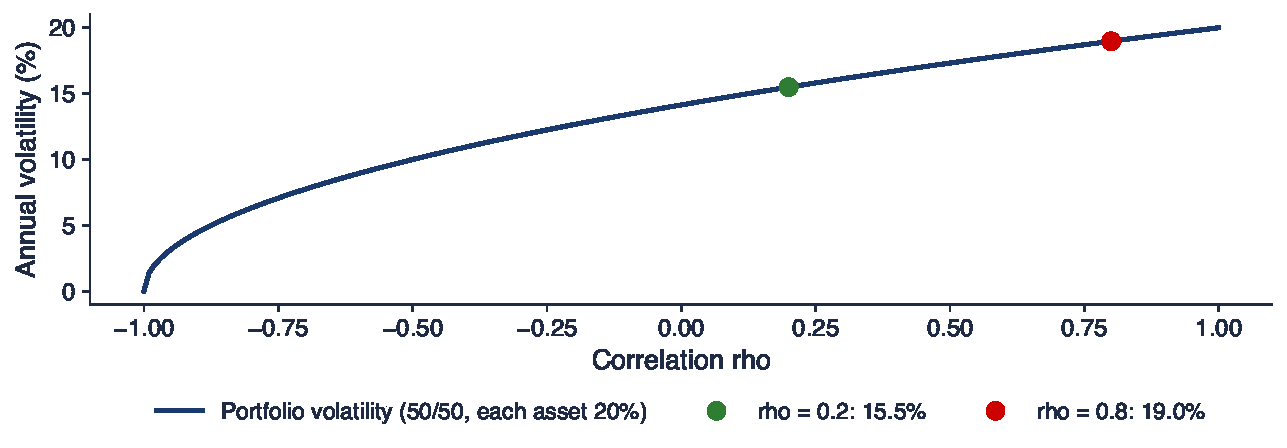
\includegraphics[width=0.97\textwidth,height=0.6\textheight,keepaspectratio]{tsa_ch14_diversification.pdf}
\end{center}
\vspace{-0.25cm}
\begin{itemize}
    \item Un portofoliu 50/50 din două active cu volatilitatea de 20\% fiecare; punctele sînt cele două cazuri din exemplul rezolvat
\end{itemize}
\quantlet{TSA\_ch14\_correlations}{\qlurl{TSA_ch14_correlations}}
\end{frame}

\begin{frame}{Interpretarea curbei de diversificare}
\itemsize{\small}
\begin{itemize}
    \item $\rho = 1$: nicio diversificare, $\sigma_p = 20\%$; $\rho = 0$: $\sigma_p = 20/\sqrt{2} \approx 14{,}1\%$; $\rho = -1$: riscul dispare
    \item Curba este concavă: o creștere a lui $\rho$ de la 0,2 la 0,8 duce volatilitatea de la 15{,}5\% la 19{,}0\%
    \item Întrebarea capitolului: rămîne $\rho$ constant pe piețele reale sau se mișcă odată cu starea pieței?
\end{itemize}
\end{frame}

\begin{frame}{Corelațiile se schimbă în timp}
\itemsize{\footnotesize}
\begin{center}
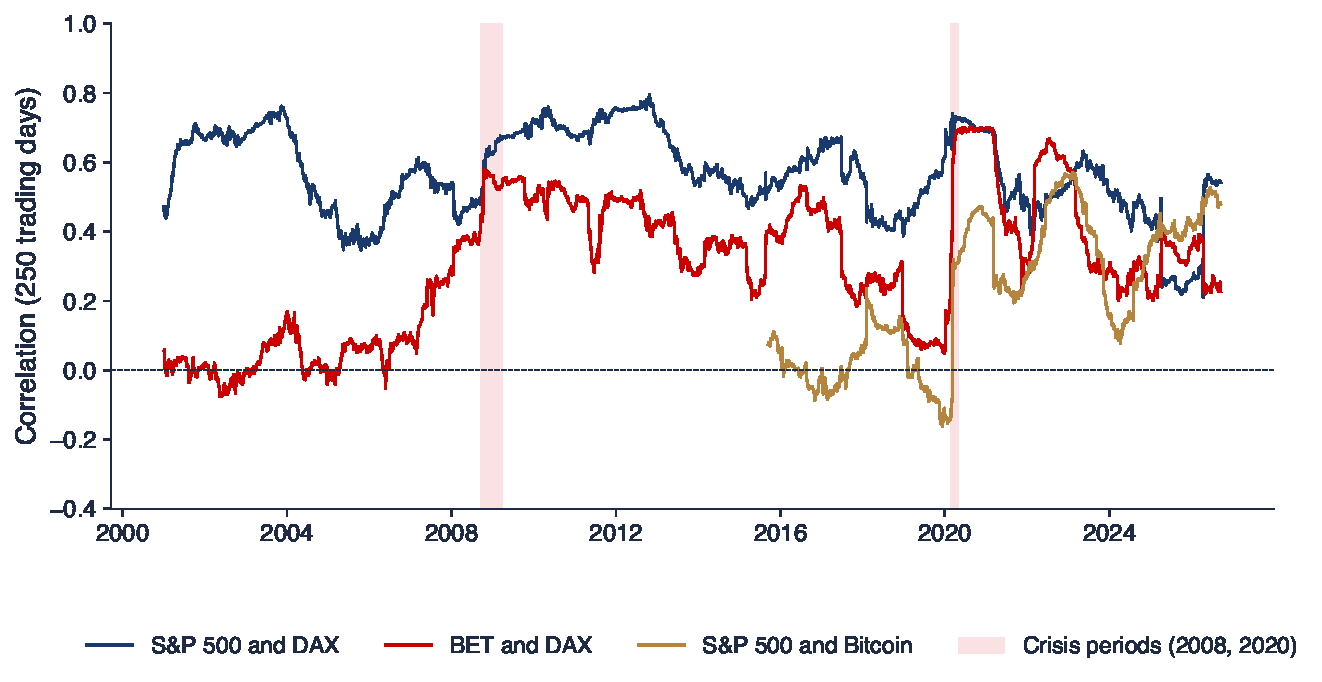
\includegraphics[width=0.97\textwidth,height=0.62\textheight,keepaspectratio]{tsa_ch14_rolling_corr.pdf}
\end{center}
\vspace{-0.25cm}
\begin{itemize}
    \item Corelația randamentelor logaritmice zilnice pe ferestre mobile de 250 de zile de tranzacționare (aproximativ un an), datată la sfîrșitul ferestrei; randamente în zilele în care se tranzacționează ambele piețe; zonele colorate: septembrie 2008--martie 2009 și februarie--aprilie 2020
\end{itemize}
\quantlet{TSA\_ch14\_correlations}{\qlurl{TSA_ch14_correlations}}
\end{frame}

\begin{frame}{Interpretarea corelațiilor pe ferestre mobile}
\itemsize{\small}
\begin{itemize}
    \item S\&P 500 și DAX: între 0{,}21 (aprilie 2026) și 0{,}80 (octombrie 2012); valoarea pe tot eșantionul 0{,}60
    \begin{itemize}
        \item criza datoriilor din zona euro din 2010--2012 a legat cele două piețe chiar mai strîns decît 2008
    \end{itemize}
    \item BET și DAX: aproape de zero înainte de 2007 (minimum $-$0{,}08), pînă la 0{,}70 în august 2020: piața românească s-a integrat cu Europa după aderarea la UE
    \item S\&P 500 și Bitcoin: de la $-$0{,}16 (decembrie 2019) la 0{,}57 (februarie 2023); Bitcoin a devenit după 2020 un activ riscant, corelat cu acțiunile
    \item Corelațiile se îndepărtează mult de orice valoare constantă: modelul trebuie să le permită să se miște
\end{itemize}
\end{frame}

\begin{frame}{O capcană: tranzacționarea asincronă}
\itemsize{\footnotesize}
\begin{itemize}
    \item Piețele se închid la ore diferite: București la 16:45 CET (17:45, ora locală), Frankfurt la 17:30 CET, New York la 22:00 CET; Bitcoin se tranzacționează non-stop
    \begin{itemize}
        \item o știre care apare după închiderea piețelor europene intră în prețurile europene abia a doua zi
    \end{itemize}
    \item Exemplu: 9 aprilie 2025, suspendarea tarifelor vamale ale SUA, anunțată după-amiaza la New York
    \begin{itemize}
        \item 9 aprilie: S\&P 500 +9{,}1\%, DAX $-$3{,}1\%; 10 aprilie: S\&P 500 $-$3{,}5\%, DAX +4{,}4\%
        \item aceeași știre, în două zile diferite: corelația zilnică este deplasată spre zero
    \end{itemize}
    \item Corelațiile randamentelor zilnice și săptămînale din 2015: S\&P 500 și BET 0{,}32 față de 0{,}46; S\&P 500 și DAX 0{,}56 față de 0{,}68; BET și DAX 0{,}42 față de 0{,}47
    \begin{itemize}
        \item diferența este mică pentru BET și DAX, care se închid aproape simultan; remedii: randamente săptămînale sau randamente între momente sincrone
    \end{itemize}
\end{itemize}
\end{frame}

\begin{frame}{Recapitulare: de ce volatilitate multivariată}
\itemsize{\small}
\begin{itemize}
    \item Varianța portofoliului $\mathbf{w}^\top\mathbf{H}\mathbf{w}$, rapoartele de acoperire și contagiunea depind toate de covarianțe
    \item Corelațiile pe ferestre mobile se mișcă mult pe piețele reale: integrare, crize, clase noi de active
    \item Verificați orele de tranzacționare: închiderile asincrone deplasează corelațiile zilnice spre zero
\end{itemize}
\end{frame}


%=============================================================================
\section{Cadrul GARCH multivariat}
%=============================================================================

\begin{frame}{Modelul pentru $N$ serii de randamente}
\itemsize{\small}
\begin{itemize}
    \item $\mathbf{r}_t = \boldsymbol{\mu} + \boldsymbol{\varepsilon}_t$, \quad $\boldsymbol{\varepsilon}_t = \mathbf{H}_t^{1/2}\boldsymbol{\eta}_t$, \quad $\boldsymbol{\eta}_t$ i.i.d. cu media $\mathbf{0}$ și covarianța $\mathbf{I}_N$
    \begin{itemize}
        \item $\mathbf{r}_t$: vectorul celor $N$ randamente din ziua $t$; $\boldsymbol{\mu}$: mediile (sau un model VAR pentru medie, \tsachlink{https://danpele.github.io/Time-Series-Analysis/RO/Cursuri/capitol6_modele_var_cauzalitate_granger.pdf}{Capitolul 6})
        \item $\mathbf{H}_t^{1/2}$: o rădăcină pătrată a lui $\mathbf{H}_t$, de exemplu factorul Cholesky $\mathbf{L}_t$, cu $\mathbf{L}_t\mathbf{L}_t^\top = \mathbf{H}_t$
    \end{itemize}
    \item $\mathbf{H}_t = \Var(\mathbf{r}_t \mid \mathcal{F}_{t-1})$: \textbf{matricea de covarianță condiționată}, dată fiind informația $\mathcal{F}_{t-1}$ pînă în ziua $t-1$
    \begin{itemize}
        \item diagonala: varianțele condiționate $h_{ii,t} = \sigma_{i,t}^2$ (\tsachlink{https://danpele.github.io/Time-Series-Analysis/RO/Cursuri/capitol5_volatilitate_conditionata_garch.pdf}{Capitolul 5})
        \item în afara diagonalei: covarianțele condiționate $h_{ij,t}$; corelația condiționată este $\rho_{ij,t} = h_{ij,t}/\sqrt{h_{ii,t}h_{jj,t}}$
    \end{itemize}
    \item Un model \textbf{GARCH multivariat} (MGARCH) este o regulă care calculează $\mathbf{H}_t$ din șocurile trecute $\boldsymbol{\varepsilon}_{t-1}$ și din $\mathbf{H}_{t-1}$
\end{itemize}
\end{frame}

\begin{frame}{Două condiții pentru $\mathbf{H}_t$}
\itemsize{\small}
\begin{itemize}
    \item \textbf{Simetria}: $h_{ij,t} = h_{ji,t}$, deci doar $N(N+1)/2$ elemente sînt distincte
    \begin{itemize}
        \item operatorul $\mathrm{vech}$ așază triunghiul inferior într-un vector: $\mathrm{vech}\begin{pmatrix} h_{11} & h_{12}\\ h_{12} & h_{22}\end{pmatrix} = (h_{11}, h_{12}, h_{22})^\top$
        \item $N = 2$: 3 elemente; $N = 10$: 55; $N = 50$: 1\,275
    \end{itemize}
    \item \textbf{Pozitiv definirea}: $\mathbf{w}^\top\mathbf{H}_t\mathbf{w} > 0$ pentru orice $\mathbf{w} \neq \mathbf{0}$, adică orice portofoliu are varianță pozitivă
    \begin{itemize}
        \item $N = 2$: $h_{11,t} > 0$ și $h_{11,t}h_{22,t} - h_{12,t}^2 > 0$, adică $|\rho_{12,t}| < 1$
        \item exemplu: $h_{11} = 4$, $h_{22} = 1$, $h_{12} = 2{,}5$ dau $4 - 6{,}25 < 0$: o „corelație” imposibilă, de 1,25
    \end{itemize}
    \item Un model MGARCH bun garantează ambele condiții pentru \textbf{orice} $t$, cu puțini parametri
\end{itemize}
\end{frame}

\begin{frame}{Estimarea prin verosimilitate maximă}
\itemsize{\small}
\begin{itemize}
    \item Dacă $\boldsymbol{\eta}_t$ urmează distribuția Normală multivariată, logaritmul verosimilității este
    \begin{itemize}
        \item $\ell(\theta) = -\frac12\sum_{t=1}^{T}\left(N\log 2\pi + \log|\mathbf{H}_t| + \boldsymbol{\varepsilon}_t^\top\mathbf{H}_t^{-1}\boldsymbol{\varepsilon}_t\right)$
        \item $|\mathbf{H}_t|$ este determinantul; pentru $N = 1$ regăsim verosimilitatea GARCH din \tsachlink{https://danpele.github.io/Time-Series-Analysis/RO/Cursuri/capitol5_volatilitate_conditionata_garch.pdf}{Capitolul 5}
    \end{itemize}
    \item Randamentele au cozi groase, deci verosimilitatea Normală este folosită ca \textbf{cvasi-verosimilitate maximă} (QML): estimatorii rămîn consistenți, iar erorile standard au nevoie de o corecție robustă (sandwich)
    \item Fiecare evaluare a lui $\ell(\theta)$ cere $\mathbf{H}_t^{-1}$ și $|\mathbf{H}_t|$ pentru toți $t$: costul crește repede cu $N$ și cu numărul de parametri
\end{itemize}
\end{frame}

\begin{frame}{Recapitulare: cadrul GARCH multivariat}
\itemsize{\small}
\begin{itemize}
    \item $\mathbf{H}_t$: varianțele condiționate pe diagonală, covarianțele în afara ei; $\rho_{ij,t} = h_{ij,t}/\sqrt{h_{ii,t}h_{jj,t}}$
    \item Condiții: simetria ($N(N+1)/2$ elemente distincte) și pozitiv definirea
    \item Estimare prin (cvasi-)verosimilitate maximă cu densitatea Normală multivariată
\end{itemize}
\end{frame}


%=============================================================================
\section{Modelele VEC și BEKK}
%=============================================================================

\begin{frame}{Modelul VEC}
\itemsize{\small}
\begin{itemize}
    \item \refBEW: fiecare element al lui $\mathbf{H}_t$ depinde de toate pătratele și produsele încrucișate ale șocurilor trecute și de toate elementele lui $\mathbf{H}_{t-1}$
    \begin{itemize}
        \item VEC(1,1): $\mathrm{vech}(\mathbf{H}_t) = \mathbf{c} + \mathbf{A}\,\mathrm{vech}(\boldsymbol{\varepsilon}_{t-1}\boldsymbol{\varepsilon}_{t-1}^\top) + \mathbf{B}\,\mathrm{vech}(\mathbf{H}_{t-1})$
        \item cu $k = N(N+1)/2$: $\mathbf{c}$ are $k$ elemente, $\mathbf{A}$ și $\mathbf{B}$ sînt $k \times k$: în total $k + 2k^2$ parametri
    \end{itemize}
    \item $N = 2$: $k = 3$ și 21 de parametri; $N = 10$: 6\,105
    \begin{itemize}
        \item iar pozitiv definirea lui $\mathbf{H}_t$ \textbf{nu} este garantată: cere restricții complicate
    \end{itemize}
    \item \textbf{VEC diagonal}: $h_{ij,t} = c_{ij} + a_{ij}\varepsilon_{i,t-1}\varepsilon_{j,t-1} + b_{ij}h_{ij,t-1}$
    \begin{itemize}
        \item fiecare element este un GARCH(1,1) separat; $3k$ parametri (9 pentru $N = 2$); tot fără garanția pozitiv definirii
    \end{itemize}
\end{itemize}
\end{frame}

\begin{frame}{Modelul BEKK}
\itemsize{\footnotesize}
\begin{itemize}
    \item \refEK: $\mathbf{H}_t = \mathbf{C}\mathbf{C}^\top + \mathbf{A}^\top\boldsymbol{\varepsilon}_{t-1}\boldsymbol{\varepsilon}_{t-1}^\top\mathbf{A} + \mathbf{B}^\top\mathbf{H}_{t-1}\mathbf{B}$
    \begin{itemize}
        \item BEKK: Baba, Engle, Kraft și Kroner; $\mathbf{C}$ inferior triunghiulară, $\mathbf{A}$ și $\mathbf{B}$ de dimensiune $N \times N$
    \end{itemize}
    \item \textbf{Pozitiv definită prin construcție}: fiecare termen este un „pătrat” $\mathbf{X}^\top\mathbf{M}\mathbf{X}$ al unei matrice pozitiv (semi)definite
    \begin{itemize}
        \item parametri: $N(N+1)/2 + 2N^2$, adică 11 pentru $N = 2$ și 255 pentru $N = 10$
    \end{itemize}
    \item \textbf{BEKK diagonal} ($\mathbf{A}$, $\mathbf{B}$ diagonale): $h_{12,t} = c_{12}^* + a_{11}a_{22}\,\varepsilon_{1,t-1}\varepsilon_{2,t-1} + b_{11}b_{22}\,h_{12,t-1}$
    \begin{itemize}
        \item \textbf{BEKK scalar}: $\mathbf{A} = a\mathbf{I}$, $\mathbf{B} = b\mathbf{I}$, aceeași dinamică pentru toate elementele
    \end{itemize}
    \item Elementele din afara diagonalei ale unei matrice $\mathbf{A}$ complete măsoară \textbf{transmiterea volatilității}: un șoc al activului 1 crește varianța activului 2
\end{itemize}
\end{frame}

\begin{frame}{Exemplu rezolvat: un pas al unui BEKK diagonal}
\itemsize{\small}
\begin{itemize}
    \item Date: $c_{12}^* = 0{,}02$, $a_{11} = 0{,}30$, $a_{22} = 0{,}25$, $b_{11} = 0{,}94$, $b_{22} = 0{,}95$, $h_{12,t-1} = 0{,}5$; șocurile de ieri $\varepsilon_{1,t-1} = -2$, $\varepsilon_{2,t-1} = -1{,}5$
    \item Pasul 1: coeficienții $a_{11}a_{22} = 0{,}075$ și $b_{11}b_{22} = 0{,}893$
    \item Pasul 2: produsul șocurilor $\varepsilon_{1,t-1}\varepsilon_{2,t-1} = 3{,}000$ (ambele negative: o scădere comună)
    \item Pasul 3: $h_{12,t} = 0{,}020 + 0{,}075 \cdot 3{,}000 + 0{,}893 \cdot 0{,}5 = 0{,}020 + 0{,}225 + 0{,}4465 = 0{,}6915$
    \item O scădere comună crește covarianța de la 0,5 la 0{,}6915; un șoc cu semne opuse ar fi scăzut-o
    \begin{itemize}
        \item observație: un BEKK diagonal nu are transmitere a volatilității, deoarece $a_{12} = a_{21} = 0$
    \end{itemize}
\end{itemize}
\end{frame}

\begin{frame}{Problema dimensionalității}
\itemsize{\footnotesize}
\begin{center}
\small
\begin{tabular}{lrrrr}
\toprule
\textbf{Model} & $N = 2$ & $N = 5$ & $N = 10$ & $N = 50$ \\
\midrule
VEC(1,1) & 21 & 465 & 6\,105 & 3\,252\,525 \\
VEC diagonal & 9 & 45 & 165 & 3\,825 \\
BEKK(1,1) & 11 & 65 & 255 & 6\,275 \\
BEKK diagonal & 7 & 25 & 75 & 1\,375 \\
BEKK scalar & 5 & 17 & 57 & 1\,277 \\
CCC & 7 & 25 & 75 & 1\,375 \\
DCC & 9 & 27 & 77 & 1\,377 \\
\bottomrule
\end{tabular}
\end{center}
\begin{itemize}
    \item Numărul de parametri ai ecuației de varianță (mediile $\boldsymbol{\mu}$ nu sînt numărate); CCC și DCC: 3 parametri GARCH pe activ, plus cele $N(N-1)/2$ corelații, iar DCC încă 2
    \item Un VEC complet pentru 50 de active are mai mulți parametri decît numărul de observații al oricărui eșantion
\end{itemize}
\end{frame}

\begin{frame}{Numărul de parametri în funcție de numărul de active}
\itemsize{\footnotesize}
\begin{center}
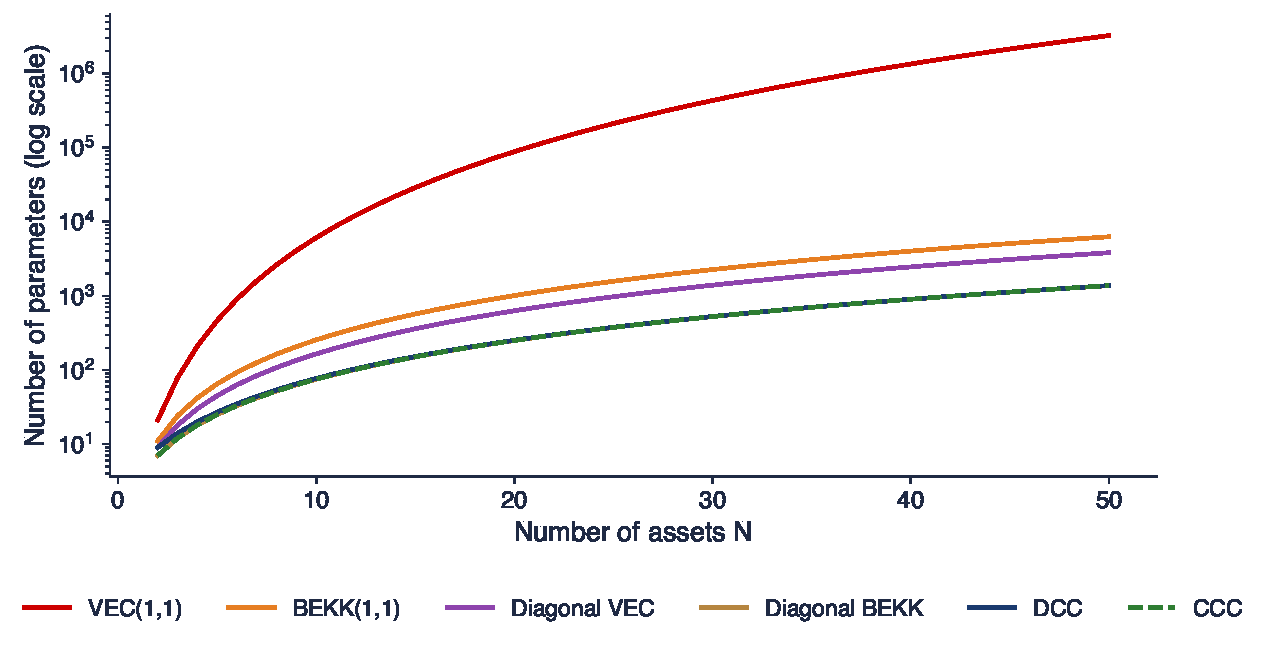
\includegraphics[width=0.97\textwidth,height=0.62\textheight,keepaspectratio]{tsa_ch14_param_count.pdf}
\end{center}
\vspace{-0.25cm}
\begin{itemize}
    \item Numărul de parametri ai ecuației de varianță pentru $N = 2, \dots, 50$ de active, scară logaritmică
\end{itemize}
\quantlet{TSA\_ch14\_parameters}{\qlurl{TSA_ch14_parameters}}
\end{frame}

\begin{frame}{Interpretarea numărului de parametri}
\itemsize{\small}
\begin{itemize}
    \item VEC crește ca $N^4/2$, BEKK complet ca $2N^2$: ambele devin imposibil de estimat dincolo de cîteva active
    \item CCC și DCC cresc ca $N^2/2$, dar corelațiile \textbf{nu} se obțin prin optimizare numerică: ele sînt corelații de selecție (secțiunea 4)
    \begin{itemize}
        \item optimizarea DCC lucrează doar cu 2 parametri, $a$ și $b$, oricare ar fi $N$
    \end{itemize}
    \item Prețul parcimoniei: toate perechile au aceeași dinamică a corelației
\end{itemize}
\end{frame}

\begin{frame}{Recapitulare: VEC și BEKK}
\itemsize{\small}
\begin{itemize}
    \item VEC: cel mai general model liniar; $k + 2k^2$ parametri, fără garanția pozitiv definirii
    \item BEKK: pozitiv definit prin construcție; elementele $a_{ij}$ din afara diagonalei măsoară transmiterea volatilității
    \item Versiunile diagonală și scalară reduc numărul de parametri, dar elimină transmiterea volatilității
\end{itemize}
\end{frame}


%=============================================================================
\section{Corelații condiționate constante și dinamice}
%=============================================================================

\begin{frame}{Separarea volatilităților de corelații}
\itemsize{\small}
\begin{itemize}
    \item Descompunerea: $\mathbf{H}_t = \mathbf{D}_t\mathbf{R}_t\mathbf{D}_t$, \quad $\mathbf{D}_t = \mathrm{diag}(\sigma_{1,t}, \dots, \sigma_{N,t})$
    \begin{itemize}
        \item $\mathbf{R}_t$: matricea corelațiilor condiționate (cu 1 pe diagonală); element cu element: $h_{ij,t} = \rho_{ij,t}\,\sigma_{i,t}\sigma_{j,t}$
        \item fiecare $\sigma_{i,t}$ este un GARCH(1,1) univariat \refBollG: $\sigma_{i,t}^2 = \omega_i + \alpha_i\varepsilon_{i,t-1}^2 + \beta_i\sigma_{i,t-1}^2$
    \end{itemize}
    \item \textbf{Reziduurile standardizate}: $z_{i,t} = \varepsilon_{i,t}/\sigma_{i,t}$; matricea lor de covarianță condiționată este chiar $\mathbf{R}_t$
    \item \textbf{CCC} (corelație condiționată constantă, \refBoll): $\mathbf{R}_t = \mathbf{R}$ pentru orice $t$
    \begin{itemize}
        \item $\mathbf{H}_t$ este pozitiv definită ori de cîte ori $\mathbf{R}$ este; $\mathbf{R}$ se estimează prin corelația de selecție a lui $z_{i,t}$
        \item covarianțele se mișcă totuși, dar numai prin volatilități; corelațiile pe ferestre mobile din secțiunea 1 contrazic această ipoteză
    \end{itemize}
\end{itemize}
\end{frame}

\begin{frame}{Robert Engle și modelul DCC}
\itemsize{\footnotesize}
\begin{columns}[T]
\begin{column}{0.33\textwidth}
\centering

\includegraphics[height=0.42\textheight]{ch5_robert_engle_2022.jpg}\\[1mm]
\imgcap{Robert F. Engle (n.\ 1942), Premiul Nobel 2003}
\imgcredit{https://commons.wikimedia.org/wiki/File:0603-Kraneshares_KRBN-RobertEngle-JonDemske-16_(cropped).jpg}{Foto: Jon Demske (2022); CC BY-SA 4.0; Wikimedia Commons}
\end{column}
\begin{column}{0.65\textwidth}
\begin{itemize}
    \item \refEngle: corelațiile urmează o recurență de tip GARCH
    \begin{itemize}
        \item $\mathbf{Q}_t = (1 - a - b)\,\bar{\mathbf{Q}} + a\,\mathbf{z}_{t-1}\mathbf{z}_{t-1}^\top + b\,\mathbf{Q}_{t-1}$
        \item $\rho_{ij,t} = q_{ij,t}/\sqrt{q_{ii,t}\,q_{jj,t}}$: rescalarea pune 1 pe diagonală
    \end{itemize}
    \item $\bar{\mathbf{Q}}$: corelația necondiționată a lui $\mathbf{z}_t$, fixată la valoarea de selecție (\textbf{țintirea corelației})
    \begin{itemize}
        \item $a \ge 0$: reacția la șocul comun de ieri; $b \ge 0$: persistența; $a + b < 1$: revenire la $\bar{\mathbf{Q}}$
    \end{itemize}
    \item $a = b = 0$ readuce modelul CCC
\end{itemize}
\end{column}
\end{columns}
\end{frame}

\begin{frame}{Estimarea în doi pași}
\itemsize{\footnotesize}
\begin{itemize}
    \item Logaritmul verosimilității se descompune într-o parte de volatilitate și o parte de corelație: $\ell = \ell_V(\theta_1) + \ell_C(\theta_1, a, b)$
    \item \textbf{Pasul 1}: estimați cîte un GARCH(1,1) pentru fiecare serie separat (\tsachlink{https://danpele.github.io/Time-Series-Analysis/RO/Cursuri/capitol5_volatilitate_conditionata_garch.pdf}{Capitolul 5}); păstrați $\hat\sigma_{i,t}$ și $\hat z_{i,t} = \hat\varepsilon_{i,t}/\hat\sigma_{i,t}$
    \item \textbf{Pasul 2}: fixați $\bar{\mathbf{Q}}$ la corelația de selecție a lui $\hat{\mathbf{z}}_t$ și maximizați doar după $(a, b)$
    \begin{itemize}
        \item $\ell_C(a, b) = -\frac12\sum_t\left(\log|\mathbf{R}_t| + \hat{\mathbf{z}}_t^\top\mathbf{R}_t^{-1}\hat{\mathbf{z}}_t - \hat{\mathbf{z}}_t^\top\hat{\mathbf{z}}_t\right)$
    \end{itemize}
    \item Estimatorul este consistent, rapid și funcționează pentru $N$ mare; erorile standard din pasul 2 ignoră eroarea de estimare din pasul 1 (sînt prea mici)
    \item \textbf{Test față de CCC}: raportul de verosimilitate $LR = 2(\ell_C^{DCC} - \ell_C^{CCC})$, comparat cu $\chi^2(2)$ (valoarea critică la 5\%: 5{,}99); vezi și \refTse
    \begin{itemize}
        \item $a = b = 0$ se află pe frontiera spațiului parametrilor, deci valoarea critică $\chi^2(2)$ este conservatoare
    \end{itemize}
\end{itemize}
\end{frame}

\begin{frame}{Exemplu rezolvat: un pas al recurenței DCC}
\itemsize{\footnotesize}
\begin{itemize}
    \item Date: $a = 0{,}05$, $b = 0{,}93$, $\bar q_{12} = 0{,}5$ (și $\bar q_{11} = \bar q_{22} = 1$), $\mathbf{Q}_{t-1} = \begin{pmatrix}1 & 0{,}5\\ 0{,}5 & 1\end{pmatrix}$, ieri $z_{1,t-1} = -2$, $z_{2,t-1} = -2{,}5$
    \item Pasul 1: $1 - a - b = 0{,}020$
    \item Pasul 2: $q_{12,t} = 0{,}020 \cdot 0{,}5 + 0{,}05 \cdot (-2)(-2{,}5) + 0{,}93 \cdot 0{,}5 = 0{,}010 + 0{,}250 + 0{,}465 = 0{,}725$
    \item Pasul 3: $q_{11,t} = 0{,}020 + 0{,}05 \cdot 4 + 0{,}93 = 1{,}150$; \quad $q_{22,t} = 0{,}020 + 0{,}05 \cdot 6{,}25 + 0{,}93 = 1{,}2625$
    \item Pasul 4: $\rho_{12,t} = 0{,}725/\sqrt{1{,}150 \cdot 1{,}2625} = 0{,}602$
    \begin{itemize}
        \item o scădere comună mare crește corelația de mîine de la 0,50 la 0{,}602; fără pasul 3, „corelația” $q_{12,t}$ ar fi 0{,}725
    \end{itemize}
\end{itemize}
\end{frame}

\begin{frame}{Interpretarea parametrilor $a$ și $b$}
\itemsize{\small}
\begin{itemize}
    \item $a$ este coeficientul de \textbf{știri}: cît mișcă un șoc comun de o zi corelația; valori zilnice tipice: 0,01--0,05
    \item $a + b$ este \textbf{persistența}: o abatere a lui $q_{ij,t}$ de la $\bar q_{ij}$ se reduce zilnic cu factorul $a + b$
    \begin{itemize}
        \item timpul de înjumătățire: $\ln 0{,}5/\ln(a + b)$ zile; $a + b = 0{,}98$ dă 34 de zile, $0{,}99$ dă 69 de zile
    \end{itemize}
    \item Aceeași interpretare ca pentru $\alpha$ și $\alpha + \beta$ într-un GARCH(1,1) (\tsachlink{https://danpele.github.io/Time-Series-Analysis/RO/Cursuri/capitol5_volatilitate_conditionata_garch.pdf}{Capitolul 5})
    \item Variante: DCC asimetric (scăderile comune mișcă mai mult corelațiile decît creșterile comune) \refCES; DCC corectat \refAielli
\end{itemize}
\end{frame}

\begin{frame}{Recapitulare: CCC și DCC}
\itemsize{\small}
\begin{itemize}
    \item $\mathbf{H}_t = \mathbf{D}_t\mathbf{R}_t\mathbf{D}_t$: volatilități GARCH combinate cu o matrice de corelații
    \item CCC: $\mathbf{R}$ constantă; DCC: $\mathbf{Q}_t$ urmează o recurență de tip GARCH, cu parametrii $a$, $b$
    \item Doi pași: GARCH univariat, apoi $(a, b)$ cu țintirea corelației; testul LR față de CCC
\end{itemize}
\end{frame}


%=============================================================================
\section{DCC pentru S\&P 500 și DAX}
%=============================================================================

\begin{frame}{Pasul 1: două modele GARCH univariate}
\itemsize{\footnotesize}
\begin{center}
\small
\begin{tabular}{lrrrrrrr}
\toprule
\textbf{Indice} & $\mu$ & $\omega$ & $\alpha$ & $\beta$ & $\alpha + \beta$ & boltire $r_t$ & boltire $z_t$ \\
\midrule
S\&P 500 & 0{,}063 & 0{,}027 & 0{,}122 & 0{,}857 & 0{,}980 & 10{,}5 & 1{,}8 \\
DAX & 0{,}067 & 0{,}030 & 0{,}098 & 0{,}886 & 0{,}984 & 6{,}2 & 1{,}4 \\
\bottomrule
\end{tabular}
\end{center}
\begin{itemize}
    \item Randamente logaritmice zilnice în \%, 6\,605 zile comune de tranzacționare, 4 ianuarie 2000--18 septembrie 2026 (EODHD); GARCH(1,1) cu medie constantă, QML gaussian; boltire: excesul de boltire
    \item Standardizarea cu $\hat\sigma_{i,t}$ elimină cea mai mare parte a excesului de boltire, dar nu tot: cozile lui $z_t$ rămîn mai groase decît la distribuția Normală
    \item Corelația randamentelor 0{,}599; corelația reziduurilor $\bar q_{12} = 0{,}575$, estimația CCC
\end{itemize}
\end{frame}

\begin{frame}{Pasul 1: volatilitățile condiționate}
\itemsize{\footnotesize}
\begin{center}
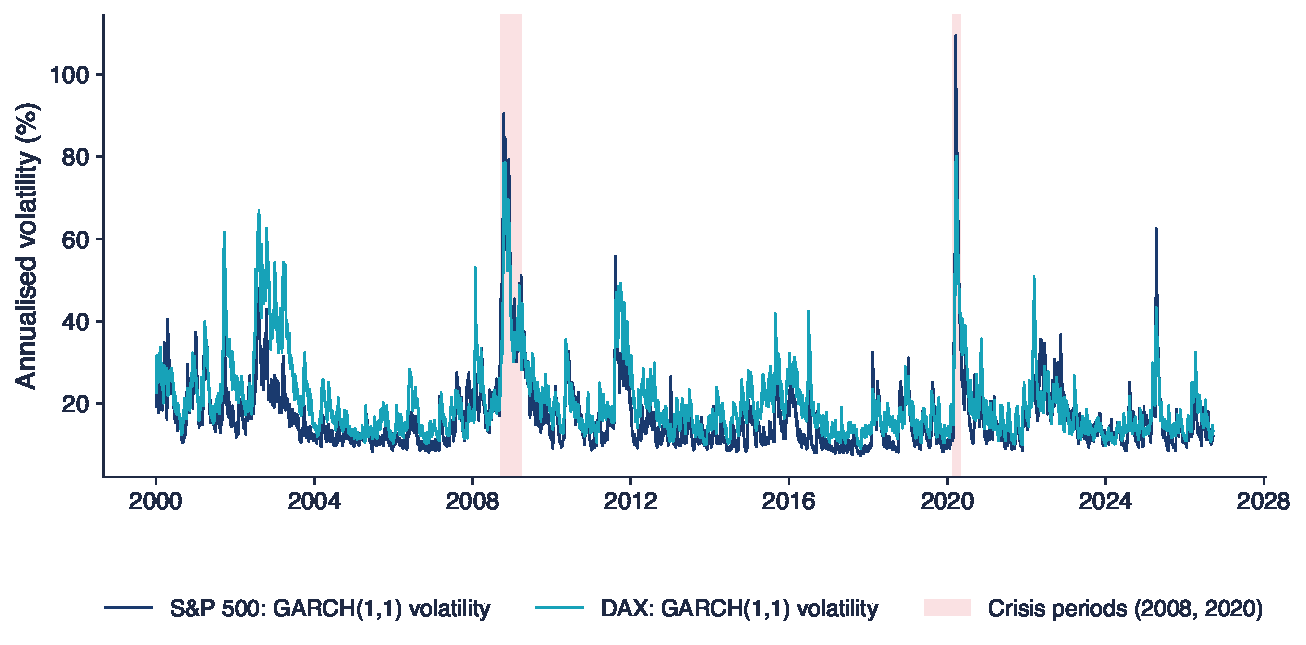
\includegraphics[width=0.97\textwidth,height=0.62\textheight,keepaspectratio]{tsa_ch14_garch_step1.pdf}
\end{center}
\vspace{-0.25cm}
\begin{itemize}
    \item Volatilitatea GARCH(1,1) prognozată cu un pas înainte, $\hat\sigma_{i,t}\sqrt{252}$, anualizată, în \%; zonele colorate: crizele din 2008 și 2020
\end{itemize}
\quantlet{TSA\_ch14\_dcc\_estimation}{\qlurl{TSA_ch14_dcc_estimation}}
\end{frame}

\begin{frame}{Interpretarea volatilităților}
\itemsize{\small}
\begin{itemize}
    \item Ambele volatilități ating maximul în aceleași săptămîni: S\&P 500 109\% pe 17 martie 2020, DAX 80\% pe 25 martie 2020
    \begin{itemize}
        \item volatility clustering apare \textbf{simultan}: covarianța crește chiar și cu o corelație constantă
    \end{itemize}
    \item Persistența 0{,}980 și 0{,}984: șocurile de volatilitate se sting lent, ca în \tsachlink{https://danpele.github.io/Time-Series-Analysis/RO/Cursuri/capitol5_volatilitate_conditionata_garch.pdf}{Capitolul 5}
    \item Pasul 2 pune o altă întrebare: după eliminarea volatilităților, este corelația rămasă constantă?
\end{itemize}
\end{frame}

\begin{frame}{Pasul 2: modelul DCC estimat}
\itemsize{\footnotesize}
\begin{center}
\small
\begin{tabular}{lrr}
\toprule
\textbf{Mărimea} & \textbf{Estimație} & \textbf{SE} \\
\midrule
$a$ & 0{,}0152 & 0{,}0035 \\
$b$ & 0{,}9766 & 0{,}0065 \\
$a + b$ & 0{,}9918 &  \\
Timpul de înjumătățire al unui șoc de corelație (zile) & 85 &  \\
LR față de CCC & 131{,}8 &  \\
Valoarea critică $\chi^2(2)$, 5\% & 5{,}99 &  \\
\bottomrule
\end{tabular}
\end{center}
\begin{itemize}
    \item $a$ este mic, dar bine determinat; $a + b$ este aproape de 1: șocurile de corelație durează luni
    \item LR = 131{,}8 este mult peste 5{,}99: corelația constantă este respinsă
    \item SE: erori standard din hessiana pasului 2 (prea mici, ignoră pasul 1)
\end{itemize}
\end{frame}

\begin{frame}{Corelația DCC dintre S\&P 500 și DAX}
\itemsize{\footnotesize}
\begin{center}
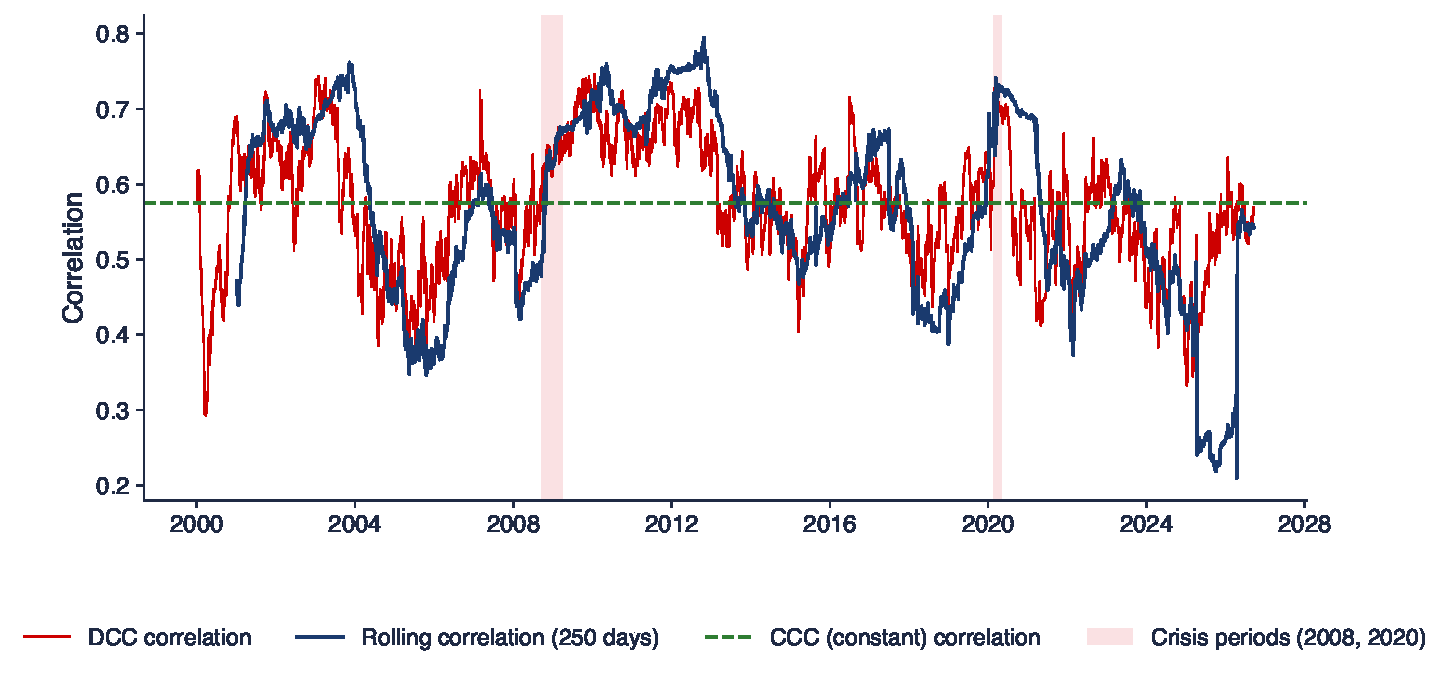
\includegraphics[width=0.97\textwidth,height=0.62\textheight,keepaspectratio]{tsa_ch14_dcc_sp_dax.pdf}
\end{center}
\vspace{-0.25cm}
\begin{itemize}
    \item Corelația DCC prognozată cu un pas înainte, $\hat\rho_{12,t}$, corelația pe ferestre mobile de 250 de zile și valoarea CCC $\bar q_{12}$; date zilnice, 4 ianuarie 2000--18 septembrie 2026
\end{itemize}
\quantlet{TSA\_ch14\_dcc\_estimation}{\qlurl{TSA_ch14_dcc_estimation}}
\end{frame}

\begin{frame}{Interpretarea corelației DCC}
\itemsize{\small}
\begin{itemize}
    \item Corelația DCC variază între 0{,}29 (martie 2000) și 0{,}75 (ianuarie 2010), în jurul unei medii de 0{,}57
    \item Urmează corelația pe ferestre mobile, dar reacționează în cîteva zile, nu într-un an, și nu cere alegerea unei ferestre
    \begin{itemize}
        \item estimarea pe ferestre mobile este mai instabilă (abaterea standard 0{,}122 față de 0{,}083) și sare cînd o zi extremă intră în fereastră sau iese din ea
    \end{itemize}
    \item Estimarea pe ferestre mobile scade brusc în 2025--2026: zilele asincrone din aprilie 2025 (secțiunea 1) o trag în jos exact 250 de zile
\end{itemize}
\end{frame}

\begin{frame}{Corelațiile în crize}
\itemsize{\footnotesize}
\begin{columns}[T]
\begin{column}{0.36\textwidth}
\centering
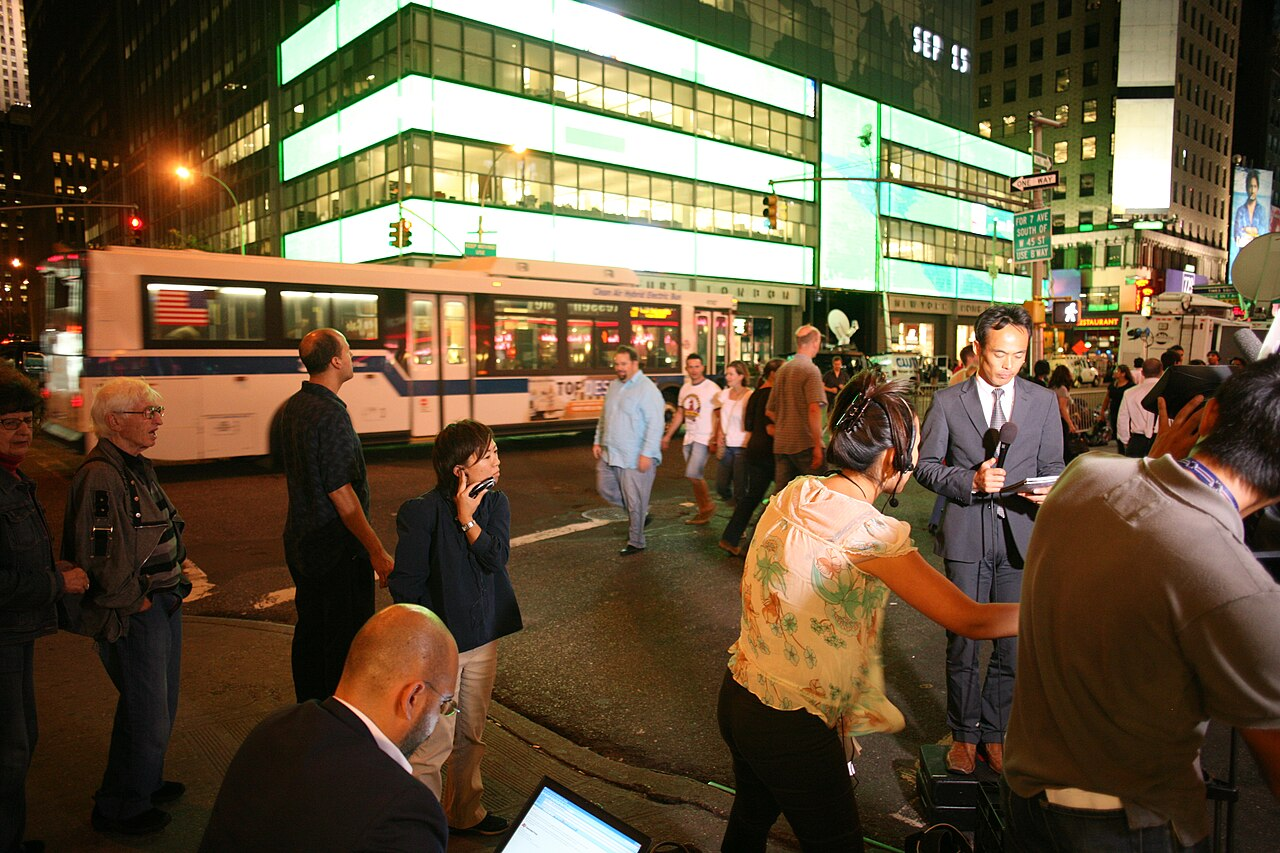
\includegraphics[height=0.36\textheight]{ch5_lehman_2008.jpg}\\[1mm]
\imgcap{Lehman Brothers, New York, 15 septembrie 2008}
\imgcredit{https://commons.wikimedia.org/wiki/File:Lehman_Brothers-NYC-20080915.jpg}{Foto: Robert Scoble (2008); CC BY 2.0; Wikimedia Commons}
\end{column}
\begin{column}{0.62\textwidth}
\begin{center}
\footnotesize
\begin{tabular}{lrr}
\toprule
\textbf{Perioada} & $\bar\rho^{DCC}$ & $\bar\sigma^{S\&P}$ (\%) \\
\midrule
Calmă, 2017--2019 & 0{,}56 & 13 \\
sept.\ 2008--martie 2009 & 0{,}63 & 51 \\
febr.--aprilie 2020 & 0{,}70 & 58 \\
\bottomrule
\end{tabular}
\end{center}
\begin{itemize}
    \item Corelația DCC medie și volatilitatea anualizată medie a S\&P 500 în fiecare perioadă
    \item Corelațiile sînt mai mari în crize, dar volatilitatea crește mult mai mult
    \item Atenție \refFR: corelația de selecție crește mecanic cînd crește volatilitatea, chiar dacă legătura nu s-a schimbat; DCC reduce acest efect, deoarece lucrează cu $z_t$, nu cu $r_t$
\end{itemize}
\end{column}
\end{columns}
\end{frame}

\begin{frame}{În interiorul crizelor din 2008 și 2020}
\itemsize{\footnotesize}
\begin{center}
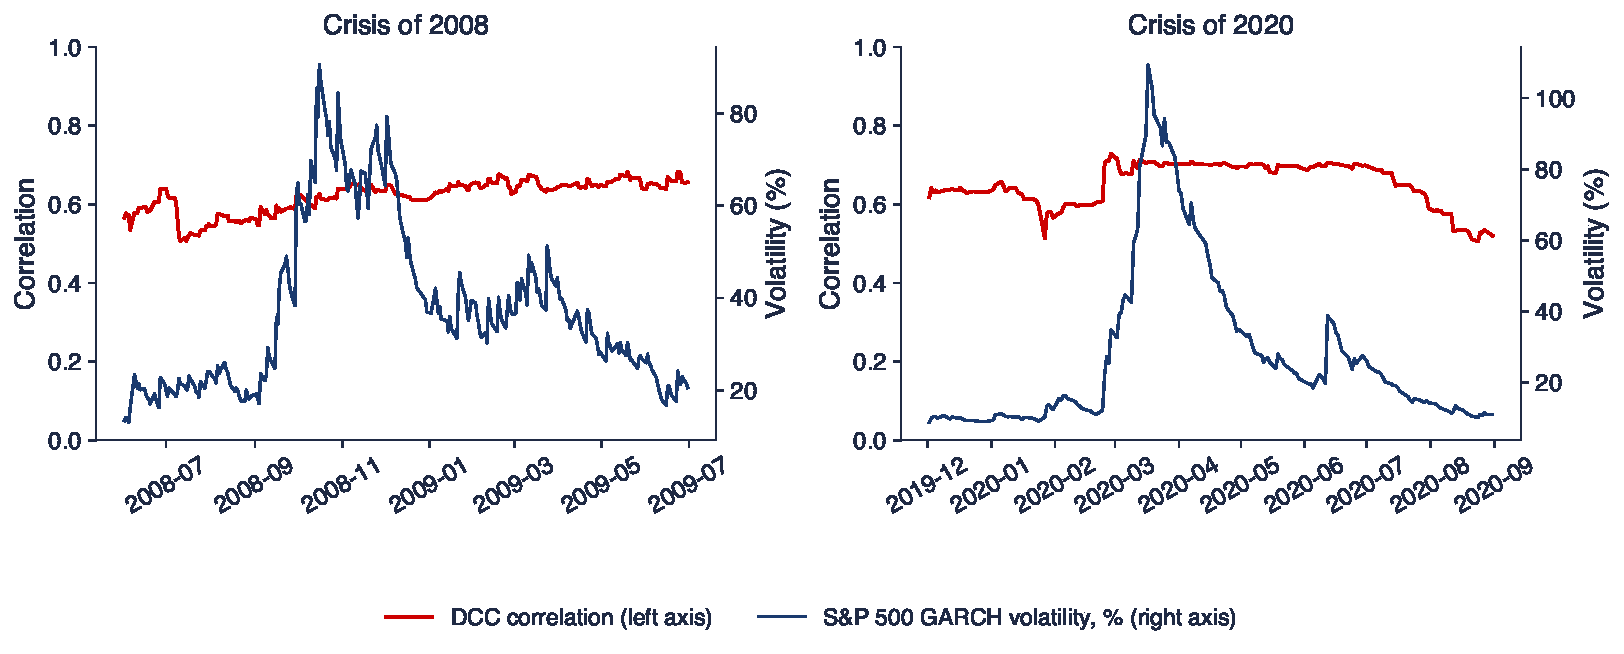
\includegraphics[width=0.97\textwidth,height=0.6\textheight,keepaspectratio]{tsa_ch14_crisis_zoom.pdf}
\end{center}
\vspace{-0.25cm}
\begin{itemize}
    \item Corelația DCC dintre S\&P 500 și DAX (axa din stînga) și volatilitatea GARCH a S\&P 500 (axa din dreapta)
\end{itemize}
\quantlet{TSA\_ch14\_dcc\_estimation}{\qlurl{TSA_ch14_dcc_estimation}}
\end{frame}

\begin{frame}{Interpretarea celor două crize}
\itemsize{\small}
\begin{itemize}
    \item 2008: volatilitatea atinge 90\% pe 16 octombrie 2008, iar corelația urcă lent de la 0{,}57 la 0{,}68 abia pe 23 iunie 2009
    \item 2020: corelația sare la 0{,}73 pe 28 februarie 2020, înaintea maximului volatilității (109\% pe 17 martie 2020)
    \begin{itemize}
        \item un șoc global a lovit ambele piețe în aceleași zile: scăderile comune alimentează recurența DCC
    \end{itemize}
    \item Corelațiile și volatilitățile nu ating neapărat maximul în același timp: modelarea lor separată, ca în DCC, arată diferența
\end{itemize}
\end{frame}

\begin{frame}{Recapitulare: S\&P 500 și DAX}
\itemsize{\small}
\begin{itemize}
    \item Pasul 1: volatilități GARCH persistente, cu maxime simultane
    \item Pasul 2: $a + b = 0{,}9918$; LR 131{,}8: corelația nu este constantă
    \item Corelații mai mari în 2008 și 2020, dar cea mai mare schimbare apare în volatilitate
\end{itemize}
\end{frame}


%=============================================================================
\section{Cinci piețe: S\&P 500, DAX, BET, EUR/RON, Bitcoin}
%=============================================================================

\begin{frame}{Un model DCC cu cinci active}
\itemsize{\footnotesize}
\begin{columns}[T]
\begin{column}{0.38\textwidth}
\centering

\includegraphics[height=0.3\textheight]{ch1_bvb_2024.jpg}\\[1mm]
\imgcap{Bursa de Valori București}
\imgcredit{https://commons.wikimedia.org/wiki/File:Bursa_de_Valori_București.jpg}{Foto: Corina Chitu (2024); CC BY-SA 4.0; Wikimedia Commons}
\end{column}
\begin{column}{0.6\textwidth}
\begin{itemize}
    \item Randamente logaritmice zilnice în cele 2\,815 zile în care se tranzacționează toate cele cinci piețe, din 6 ianuarie 2015
    \begin{itemize}
        \item EUR/RON: cursul de referință BNR (stabilit la ora 13:00, ora Bucureștiului); BET: Bursa de Valori București; Bitcoin: închiderea zilei (UTC)
    \end{itemize}
    \item Pasul 1: persistența GARCH S\&P 500 0{,}961, DAX 0{,}965, BET 0{,}941, EUR/RON 0{,}985, Bitcoin 0{,}958
    \item Pasul 2: $\hat a = 0{,}0088$ (SE 0{,}0019), $\hat b = 0{,}9782$ (SE 0{,}0062); timpul de înjumătățire 53 de zile; LR față de CCC 88{,}5
    \begin{itemize}
        \item 10 perechi de corelații, o singură pereche de parametri de dinamică $(a, b)$ pentru toate
    \end{itemize}
\end{itemize}
\end{column}
\end{columns}
\end{frame}

\begin{frame}{Corelațiile dinamice a patru perechi}
\itemsize{\footnotesize}
\begin{center}
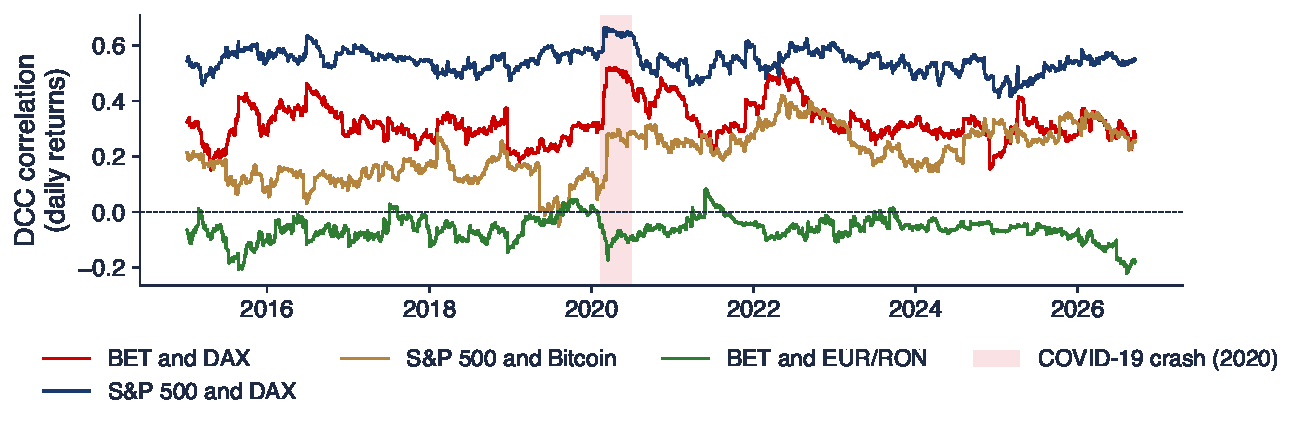
\includegraphics[width=0.97\textwidth,height=0.62\textheight,keepaspectratio]{tsa_ch14_panel_corr.pdf}
\end{center}
\vspace{-0.25cm}
\begin{itemize}
    \item Corelațiile DCC prognozate cu un pas înainte din modelul cu cinci active; zona colorată: crahul COVID-19, jumătatea lui februarie--iunie 2020
\end{itemize}
\quantlet{TSA\_ch14\_dcc\_panel}{\qlurl{TSA_ch14_dcc_panel}}
\end{frame}

\begin{frame}{Interpretarea celor patru perechi}
\itemsize{\small}
\begin{itemize}
    \item S\&P 500 și DAX: legătura cea mai puternică, media 0{,}54; BET și DAX: media 0{,}32, între 0{,}15 și 0{,}53 (aprilie 2022)
    \item S\&P 500 și Bitcoin: de la $-$0{,}05 la 0{,}42 (mai 2022); media 0{,}21
    \begin{itemize}
        \item beneficiul de diversificare al lui Bitcoin s-a redus după 2020
    \end{itemize}
    \item BET și EUR/RON: aproape de zero (media $-$0{,}06); un leu mai slab tinde să însoțească un BET mai slab, o legătură negativă mică
    \item Un singur $(a, b)$ pentru toate perechile: perechi cu viteze diferite sînt forțate la același ritm, prețul parcimoniei DCC
\end{itemize}
\end{frame}

\begin{frame}{Corelațiile medii: perioadă calmă și criză}
\itemsize{\footnotesize}
\begin{center}
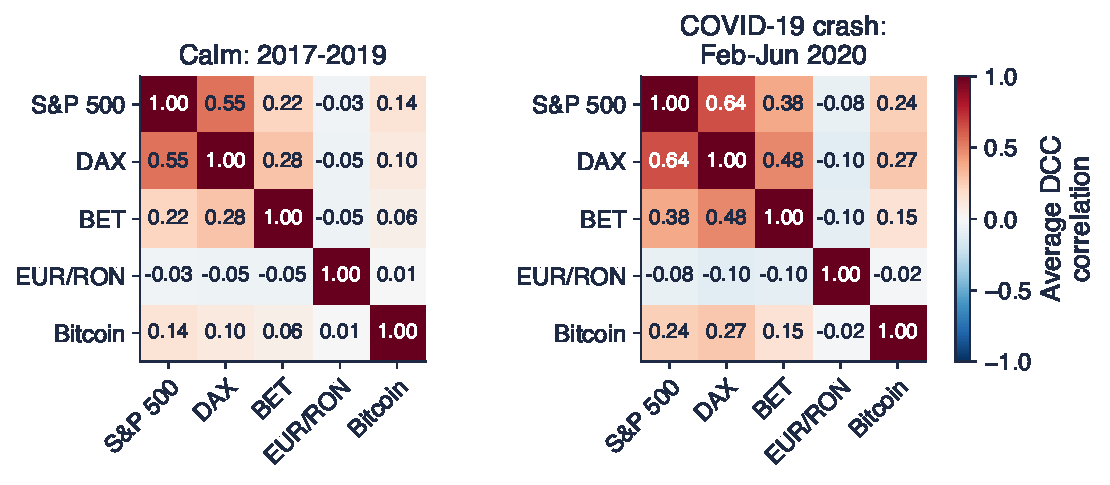
\includegraphics[width=0.97\textwidth,height=0.6\textheight,keepaspectratio]{tsa_ch14_panel_heatmap.pdf}
\end{center}
\vspace{-0.25cm}
\begin{itemize}
    \item Matricea medie a corelațiilor DCC prognozate cu un pas înainte: 2017--2019 și jumătatea lui februarie--iunie 2020 (89 de zile comune de tranzacționare)
\end{itemize}
\quantlet{TSA\_ch14\_dcc\_panel}{\qlurl{TSA_ch14_dcc_panel}}
\end{frame}

\begin{frame}{Interpretarea celor două matrice}
\itemsize{\small}
\begin{itemize}
    \item Corelația medie dintre perechi crește de la 0{,}12 la 0{,}19
    \begin{itemize}
        \item BET și DAX: 0{,}28 $\to$ 0{,}48; S\&P 500 și BET: 0{,}22 $\to$ 0{,}38; DAX și Bitcoin: 0{,}10 $\to$ 0{,}27
    \end{itemize}
    \item Cele mai mari creșteri apar pentru BET și pentru Bitcoin, slab legate de piețele mari în perioadele calme: tocmai activele care ar fi trebuit să diversifice riscul
    \item EUR/RON rămîne aproape de zero sau ușor negativ față de toate piețele de acțiuni: singurul element de diversificare din acest set
\end{itemize}
\end{frame}

\begin{frame}{Recapitulare: cinci piețe}
\itemsize{\small}
\begin{itemize}
    \item Un singur DCC pentru 5 active: 2 parametri de dinamică pentru 10 corelații
    \item Corelațiile pieței românești cu Europa și ale lui Bitcoin cu acțiunile se mișcă mult
    \item În crahul din 2020 legăturile slabe s-au întărit cel mai mult: diversificarea slăbește în crize
\end{itemize}
\end{frame}


%=============================================================================
\section{VaR 1\% al unui portofoliu cu DCC}
%=============================================================================

\begin{frame}{De la $\mathbf{H}_t$ la VaR-ul unui portofoliu}
\itemsize{\small}
\begin{itemize}
    \item Randamentul portofoliului $r_{p,t} = \mathbf{w}^\top\mathbf{r}_t$; media condiționată $\mu_p = \mathbf{w}^\top\boldsymbol{\mu}$ și volatilitatea $\sigma_{p,t} = \sqrt{\mathbf{w}^\top\mathbf{H}_t\mathbf{w}}$
    \item \textbf{VaR 1\%}: pierderea depășită cu probabilitatea 1\%, $\mathrm{VaR}_{0{,}01,t} = -q_{0{,}01}(r_{p,t}) = -(\mu_p + q\,\sigma_{p,t})$
    \begin{itemize}
        \item distribuția Normală: $q = z_{0{,}01} = -2{,}326$
        \item \textbf{simularea istorică filtrată} (FHS): $q$ = cuantila empirică de 1\% a randamentelor standardizate trecute ale portofoliului, $(r_{p,t} - \mu_p)/\sigma_{p,t}$
    \end{itemize}
    \item Trei variante pentru $\mathbf{H}_t$: DCC; CCC (volatilități GARCH cu o corelație constantă); \textbf{statică} (o singură matrice de covarianță de selecție pentru toate zilele)
\end{itemize}
\end{frame}

\begin{frame}{Exemplu rezolvat: VaR 1\% pentru două active}
\itemsize{\small}
\begin{itemize}
    \item Prognozele de azi: $\sigma_1 = 1{,}5\%$, $\sigma_2 = 1{,}2\%$ (zilnic), ponderi 50\% și 50\%, media 0
    \item Calm, $\rho_t = 0{,}3$: $\sigma_p^2 = 0{,}25 \cdot 2{,}25 + 0{,}25 \cdot 1{,}44 + 2 \cdot 0{,}25 \cdot 0{,}3 \cdot 1{,}8$, deci $\sigma_p = 1{,}092\%$ și VaR 1\% $= 2{,}326 \cdot 1{,}092 = 2{,}54\%$
    \item Criză, $\rho_t = 0{,}9$ (aceleași volatilități): $\sigma_p = 1{,}316\%$ și VaR 1\% $= 3{,}06\%$
    \begin{itemize}
        \item doar saltul corelației adaugă o cincime la VaR; într-o criză reală cresc și volatilitățile
    \end{itemize}
    \item Pentru un portofoliu de 1 milion de lei: VaR 1\% de aproximativ 25{,}4 mii de lei în perioada calmă și 30{,}6 mii de lei în cazul de criză
\end{itemize}
\end{frame}

\begin{frame}{Backtesting pentru VaR}
\itemsize{\footnotesize}
\begin{itemize}
    \item O \textbf{încălcare} în ziua $t$: $r_{p,t} < -\mathrm{VaR}_{0{,}01,t}$; un VaR 1\% corect are încălcări în 1\% din zile, la momente aleatoare
    \item \textbf{Testul Kupiec} \refKupiec\ (frecvența): $x$ încălcări în $n$ zile, $\hat p = x/n$
    \begin{itemize}
        \item $LR_{uc} = -2\log\dfrac{(1-0{,}01)^{n-x}\,0{,}01^{x}}{(1-\hat p)^{n-x}\,\hat p^{x}} \sim \chi^2(1)$; respingem la 5\% dacă $LR_{uc} > 3{,}84$
    \end{itemize}
    \item \textbf{Testul Christoffersen} \refChr\ (independența): este o încălcare mai probabilă în ziua de după o încălcare?
    \begin{itemize}
        \item compară $\pi_{11} = P(\text{încălcare} \mid \text{încălcare ieri})$ cu $\pi_{01} = P(\text{încălcare} \mid \text{fără încălcare ieri})$
    \end{itemize}
    \item \textbf{Un design corect}: estimați toți parametrii pe 2000--2014 (3\,712 de zile), apoi rulați filtrele mai departe pe 2015--2026 (2\,893 de zile), fără reestimare
\end{itemize}
\end{frame}

\begin{frame}{VaR 1\% al unui portofoliu S\&P 500 și DAX, 2015--2026}
\itemsize{\footnotesize}
\begin{center}
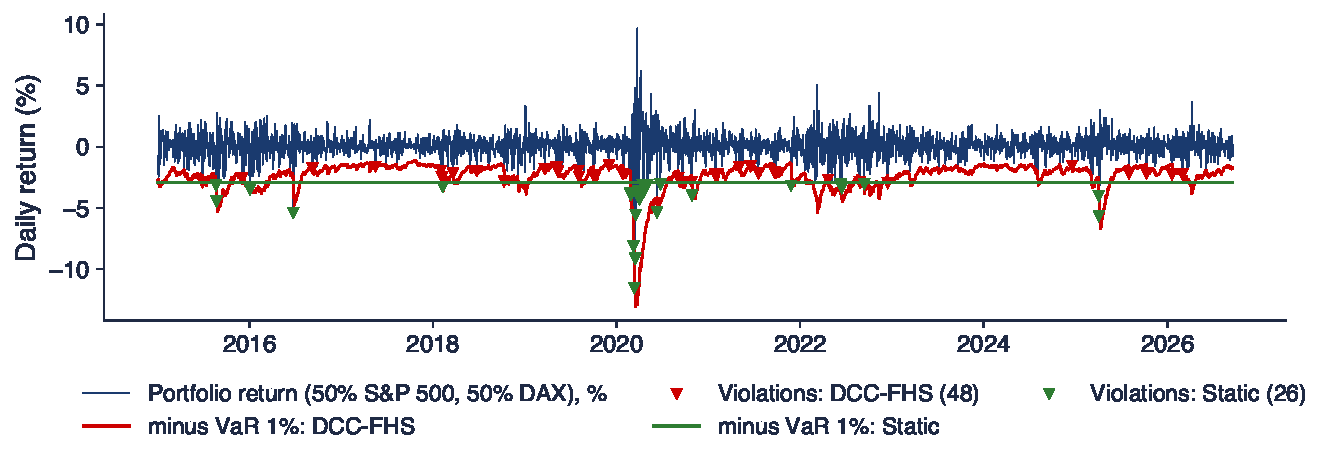
\includegraphics[width=0.97\textwidth,height=0.62\textheight,keepaspectratio]{tsa_ch14_var_backtest.pdf}
\end{center}
\vspace{-0.25cm}
\begin{itemize}
    \item Randamentul zilnic al unui portofoliu 50/50 și minus VaR 1\% din DCC cu simulare istorică filtrată și dintr-o matrice de covarianță statică; triunghiuri: încălcări
\end{itemize}
\quantlet{TSA\_ch14\_portfolio\_var}{\qlurl{TSA_ch14_portfolio_var}}
\end{frame}

\begin{frame}{Interpretarea backtesting-ului}
\itemsize{\footnotesize}
\begin{center}
\footnotesize
\begin{tabular}{lrrrrrr}
\toprule
\textbf{Model} & Încălcări & Rata & $LR_{uc}$ & $p$ & $p$ indep. & febr.--apr.\ 2020 \\
\midrule
DCC, Normală & 65 & 2{,}25\% & 33{,}6 & $<$\,0{,}001 & 0{,}003 & 4 \\
DCC, FHS & 48 & 1{,}66\% & 10{,}6 & 0{,}001 & 0{,}008 & 4 \\
CCC, Normală & 57 & 1{,}97\% & 21{,}4 & $<$\,0{,}001 & 0{,}030 & 4 \\
Statică, Normală & 26 & 0{,}90\% & 0{,}3 & 0{,}577 & 0{,}001 & 10 \\
\bottomrule
\end{tabular}
\end{center}
\begin{itemize}
    \item Așteptat: aproximativ 29 de încălcări în 2\,893 de zile
    \item Modelele dinamice cu cuantilele distribuției Normale au prea multe încălcări: reziduurile au cozi groase (\tsachlink{https://danpele.github.io/Time-Series-Analysis/RO/Cursuri/capitol5_volatilitate_conditionata_garch.pdf}{Capitolul 5}); FHS ($q = -2{,}59$) reduce rata la 1{,}66\%
    \item VaR-ul static trece testul de frecvență, dar încălcările lui se grupează: 10 doar în februarie--aprilie 2020, iar după o încălcare ziua următoare este tot o încălcare cu probabilitatea 11{,}5\%
    \item VaR-ul static este prea mare în anii calmi (2{,}95\% în fiecare zi) și mult prea mic într-un crah; un VaR dinamic se adaptează în ambele sensuri
\end{itemize}
\end{frame}

\begin{frame}{Recapitulare: VaR-ul portofoliului}
\itemsize{\small}
\begin{itemize}
    \item $\sigma_{p,t} = \sqrt{\mathbf{w}^\top\mathbf{H}_t\mathbf{w}}$; VaR 1\% $= -(\mu_p + q\,\sigma_{p,t})$
    \item Backtesting în afara eșantionului: Kupiec (frecvența) și Christoffersen (independența)
    \item Covarianțele dinamice corectează gruparea încălcărilor; cozile groase cer o cuantilă mai bună decît cea a distribuției Normale
\end{itemize}
\end{frame}


%=============================================================================
\section{Rapoarte dinamice de acoperire}
%=============================================================================

\begin{frame}{Raportul de acoperire cu varianță minimă}
\itemsize{\small}
\begin{itemize}
    \item Dețineți o unitate din activul $s$ (de exemplu acțiuni românești, BET) și vindeți $h$ unități dintr-un activ de acoperire $f$ (de exemplu un contract futures pe DAX)
    \begin{itemize}
        \item randamentul acoperit $r_{s,t} - h\,r_{f,t}$, cu varianța $\sigma_s^2 - 2h\,\sigma_{sf} + h^2\sigma_f^2$
    \end{itemize}
    \item Anulînd derivata în raport cu $h$: $h^* = \dfrac{\sigma_{sf}}{\sigma_f^2} = \rho\,\dfrac{\sigma_s}{\sigma_f}$ \refEd
    \begin{itemize}
        \item $h^*$ static: panta OLS a regresiei lui $r_s$ pe $r_f$; \textbf{dinamic}: $h_t^* = h_{sf,t}/h_{ff,t}$ dintr-un model MGARCH \refKS
    \end{itemize}
    \item \textbf{Eficiența acoperirii}: $HE = 1 - \Var(r_s - h\,r_f)/\Var(r_s)$, ponderea varianței eliminate
    \begin{itemize}
        \item cu $h = h^*$ constant: $HE = \rho^2$; o acoperire este atît de bună cît este corelația
    \end{itemize}
\end{itemize}
\end{frame}

\begin{frame}{Exemplu rezolvat: un raport de acoperire}
\itemsize{\small}
\begin{itemize}
    \item Date: $\sigma_s = 1{,}2\%$, $\sigma_f = 1{,}0\%$ (zilnic), $\rho = 0{,}8$
    \item Pasul 1: $\sigma_{sf} = \rho\,\sigma_s\sigma_f = 0{,}8 \cdot 1{,}2 \cdot 1{,}0 = 0{,}96$
    \item Pasul 2: $h^* = \sigma_{sf}/\sigma_f^2 = 0{,}96/1 = 0{,}96$: vindeți 0{,}96 unități din $f$ pentru fiecare unitate din $s$
    \item Pasul 3: $HE = \rho^2 = 0{,}64$; volatilitatea poziției acoperite este $\sigma_s\sqrt{1 - \rho^2} = 0{,}72\%$ în loc de 1,2\%
    \item Dacă mîine DCC prognozează $\rho_t = 0{,}5$ și $\sigma_{f,t} = 2\%$, raportul de acoperire devine $0{,}5 \cdot 1{,}2/2 = 0{,}3$: poziția trebuie ajustată
\end{itemize}
\end{frame}

\begin{frame}{Acoperirea BET cu DAX, 2015--2026}
\itemsize{\footnotesize}
\begin{center}
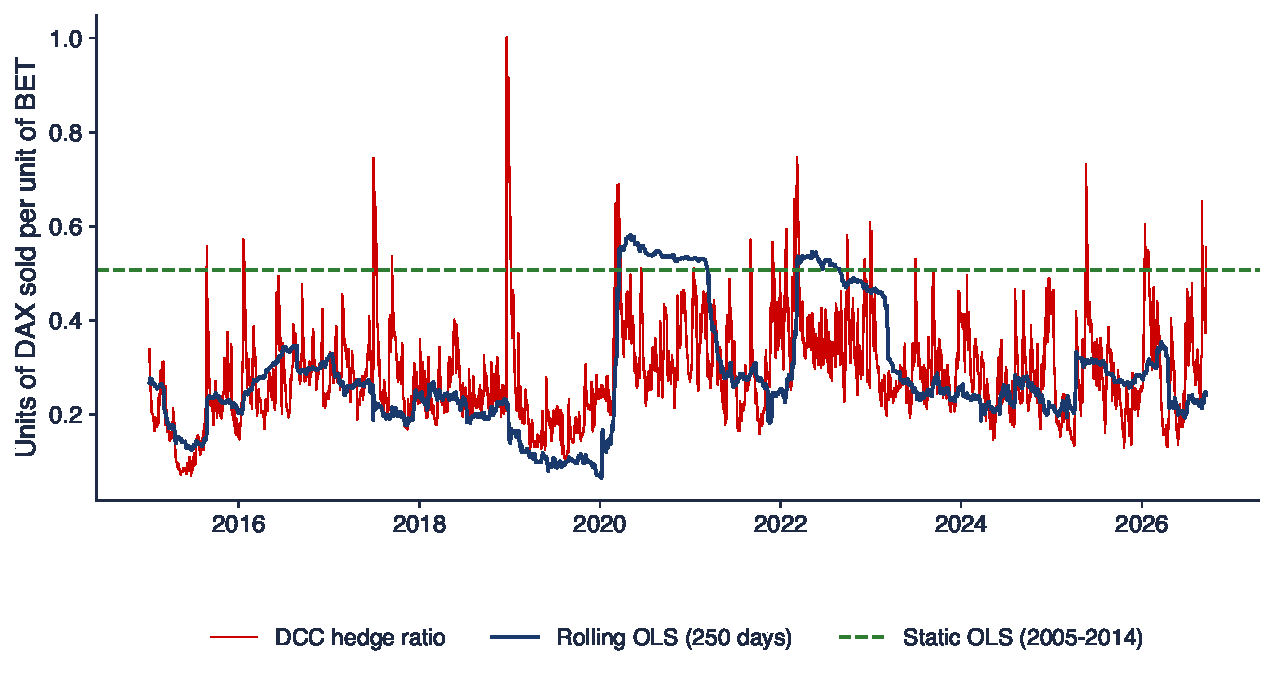
\includegraphics[width=0.97\textwidth,height=0.62\textheight,keepaspectratio]{tsa_ch14_hedge.pdf}
\end{center}
\vspace{-0.25cm}
\begin{itemize}
    \item Randamente zilnice în zilele comune de tranzacționare din 2005; toți parametrii estimați pe 2005--2014; DCC: $h_t = \hat\rho_t\hat\sigma_{BET,t}/\hat\sigma_{DAX,t}$; OLS pe ferestre mobile: panta din ultimele 250 de zile
\end{itemize}
\quantlet{TSA\_ch14\_hedging}{\qlurl{TSA_ch14_hedging}}
\end{frame}

\begin{frame}{Interpretarea rapoartelor de acoperire}
\itemsize{\small}
\begin{itemize}
    \item Raportul static 0{,}51 reflectă perioada 2005--2014, care include criza din 2008; după 2015 raportul DCC are media 0{,}29, între 0{,}07 și 1{,}00 (20 decembrie 2018)
    \item Eficiența acoperirii în afara eșantionului (2\,893 de zile): statică 13{,}6\%, OLS pe ferestre mobile 18{,}0\%, DCC 19{,}1\%
    \begin{itemize}
        \item rapoartele dinamice elimină mai mult risc, iar DCC face acest lucru fără alegerea unei ferestre
    \end{itemize}
    \item Toate valorile eficienței sînt modeste: corelația DCC dintre BET și DAX are media 0{,}32 din 2015, deci $\rho^2$ este mic
    \begin{itemize}
        \item un raport DCC zilnic implică și costuri zilnice de tranzacționare, care nu sînt incluse aici
    \end{itemize}
\end{itemize}
\end{frame}

\begin{frame}{Recapitulare: acoperirea riscului}
\itemsize{\small}
\begin{itemize}
    \item $h_t^* = h_{sf,t}/h_{ff,t} = \rho_t\sigma_{s,t}/\sigma_{f,t}$; $HE = 1 - \Var(\text{acoperit})/\Var(\text{neacoperit})$
    \item BET cu DAX: DCC 19{,}1\% față de static 13{,}6\% în afara eșantionului
    \item Evaluați o acoperire în afara eșantionului și după costurile de tranzacționare
\end{itemize}
\end{frame}


%=============================================================================
\section{Legături cu alte capitole și limite}
%=============================================================================

\begin{frame}{Legături cu \tsachlinkt{https://danpele.github.io/Time-Series-Analysis/RO/Cursuri/capitol5_volatilitate_conditionata_garch.pdf}{Capitolele 5}, \tsachlinkt{https://danpele.github.io/Time-Series-Analysis/RO/Cursuri/capitol6_modele_var_cauzalitate_granger.pdf}{6} și \tsachlinkt{https://danpele.github.io/Time-Series-Analysis/RO/Cursuri/capitol7_cointegrare_vecm.pdf}{7}}
\itemsize{\small}
\begin{itemize}
    \item \textbf{\tsachlink{https://danpele.github.io/Time-Series-Analysis/RO/Cursuri/capitol5_volatilitate_conditionata_garch.pdf}{Capitolul 5}}: orice model MGARCH conține modele GARCH univariate; în DCC ele sînt chiar pasul 1
    \item \textbf{\tsachlink{https://danpele.github.io/Time-Series-Analysis/RO/Cursuri/capitol6_modele_var_cauzalitate_granger.pdf}{Capitolul 6}}: un VAR modelează transmiterea în \textbf{medie} (de exemplu, dacă randamentul DAX de ieri ajută la prognoza randamentului BET de azi); BEKK cu $\mathbf{A}$ complet modelează transmiterea în \textbf{varianță}
    \begin{itemize}
        \item cele două se combină: un VAR pentru $\boldsymbol{\mu}_t$ și un MGARCH pentru $\mathbf{H}_t$; indicii de transmitere din descompunerea varianței \refDY
    \end{itemize}
    \item \textbf{\tsachlink{https://danpele.github.io/Time-Series-Analysis/RO/Cursuri/capitol7_cointegrare_vecm.pdf}{Capitolul 7}}: cointegrarea este o legătură pe \textbf{termen lung} între nivelurile prețurilor; corelația este o legătură pe \textbf{termen scurt} între randamente
    \begin{itemize}
        \item două prețuri pot fi puternic corelate de la o zi la alta și să se îndepărteze definitiv, sau pot fi cointegrate cu o corelație zilnică mică
        \item un VECM poate avea erori de tip DCC: echilibru în medie, corelație dinamică în șocuri
    \end{itemize}
\end{itemize}
\end{frame}

\begin{frame}{Limite și extensii}
\itemsize{\footnotesize}
\begin{columns}[T]
\begin{column}{0.34\textwidth}
\centering
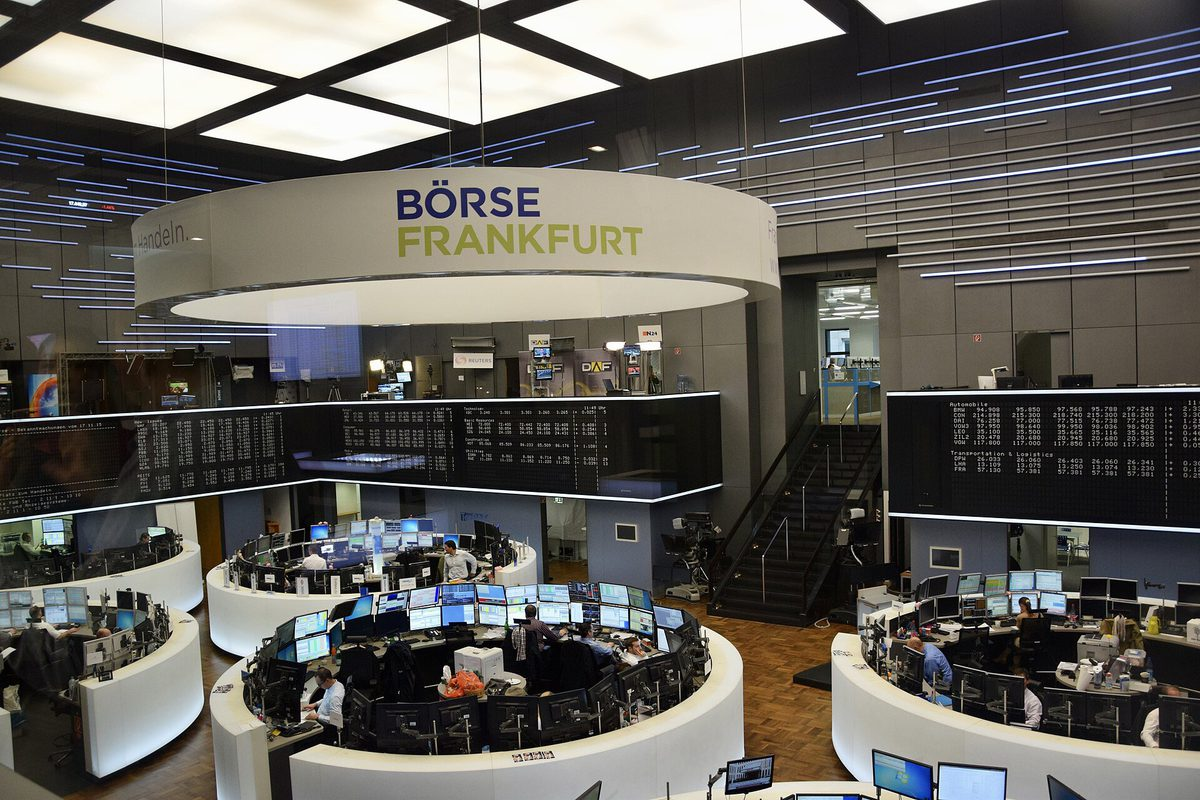
\includegraphics[height=0.3\textheight]{ch6_frankfurt_exchange_2015.jpg}\\[1mm]
\imgcap{Bursa din Frankfurt}
\imgcredit{https://commons.wikimedia.org/wiki/File:Frankfurt_Stock_Exchange_(Ank_Kumar)_01.jpg}{Foto: Ank Kumar (2015); CC BY-SA 4.0; Wikimedia Commons}
\end{column}
\begin{column}{0.64\textwidth}
\begin{itemize}
    \item Un singur $(a, b)$ pentru toate perechile; DCC nu are transmitere între volatilități
    \item QML cu distribuția Normală subestimează cozile: pentru risc folosiți inovații Student $t$ sau FHS
    \item Asimetria: corelațiile reacționează mai mult la scăderile comune (DCC asimetric, \refCES)
    \item Sute de active: modele factoriale, verosimilitate compusă și contracția (shrinkage) lui $\bar{\mathbf{Q}}$
    \item Corelația măsoară dependența liniară; pentru extreme comune vedeți copulele și dependența în cozi \refLS
\end{itemize}
\end{column}
\end{columns}
\end{frame}


%=============================================================================
\section{Contribuția posibilă a AI}
%=============================================================================

\begin{frame}{Contribuția posibilă a AI}
\itemsize{\small}
\begin{itemize}
    \item \textbf{Cod}: o primă versiune a verosimilității DCC, a unui filtru BEKK, a testului Kupiec
    \item \textbf{Explicații}: o a doua explicație a descompunerii $\mathbf{D}_t\mathbf{R}_t\mathbf{D}_t$, a țintirii corelației, a formulei raportului de acoperire
    \item \textbf{Explorare}: DCC pentru multe perechi (piețe din Europa Centrală și de Est, sectoare, valute) și comportamentul lor în crize
    \item Exemplu de prompt
    \begin{itemize}
        \item \aiprompt{Write Python code that fits a GARCH(1,1) to daily BET and DAX log returns on common trading days, estimates a DCC(1,1) model by two-step maximum likelihood with correlation targeting, plots the dynamic hedge ratio and compares its out-of-sample hedging effectiveness with static OLS.}
    \end{itemize}
\end{itemize}
\end{frame}

\begin{frame}{Verificări necesare}
\itemsize{\small}
\begin{itemize}
    \item Biblioteca: \texttt{arch} nu are model DCC; un răspuns AI care apelează \texttt{arch\_model(..., vol='DCC')} l-a inventat
    \item Momentul: $\mathbf{Q}_t$ trebuie să folosească $\mathbf{z}_{t-1}$, nu $\mathbf{z}_t$; altfel VaR-ul și acoperirea folosesc informația de mîine
    \item Rescalarea: $\rho_{ij,t} = q_{ij,t}/\sqrt{q_{ii,t}q_{jj,t}}$, iar fiecare $\mathbf{R}_t$ trebuie să aibă 1 pe diagonală și $|\rho| < 1$
    \item Calendarele: aliniați prețurile pe zilele comune de tranzacționare înainte de a calcula randamentele; atenție la închiderile asincrone
    \item Evaluarea: estimați pe o perioadă și testați pe alta; simulați un DCC cu $(a, b)$ cunoscuți și verificați că programul îi regăsește
    \item Fiecare referință citată: trebuie să existe; verificați DOI-ul
\end{itemize}
\end{frame}


%=============================================================================
\section{Rezumat}
%=============================================================================

\begin{frame}{Idei de reținut}
\itemsize{\small}
\begin{itemize}
    \item Riscul portofoliului, acoperirea și contagiunea depind de covarianțele variabile în timp $\mathbf{H}_t$
    \item VEC este general, dar are prea mulți parametri; BEKK este pozitiv definit prin construcție și măsoară transmiterea volatilității
    \item CCC și DCC descompun $\mathbf{H}_t = \mathbf{D}_t\mathbf{R}_t\mathbf{D}_t$ și se estimează în doi pași; DCC are nevoie în pasul 2 doar de $(a, b)$
    \item Corelațiile reale se mișcă: integrare, crize, active noi; corelația constantă este respinsă
    \item Aplicații: VaR 1\% al portofoliului, cu backtesting; rapoarte dinamice de acoperire evaluate în afara eșantionului
\end{itemize}
\end{frame}

\begin{frame}{Formule de reținut}
\itemsize{\small}
{\renewcommand{\arraystretch}{1.35}\begin{center}
\scriptsize
\begin{tabular}{ll}
\toprule
\textbf{Mărimea} & \textbf{Formula} \\
\midrule
Corelația & $\rho_{ij,t} = h_{ij,t}/\sqrt{h_{ii,t}h_{jj,t}}$ \\
BEKK(1,1) & $\mathbf{H}_t = \mathbf{C}\mathbf{C}^\top + \mathbf{A}^\top\boldsymbol{\varepsilon}_{t-1}\boldsymbol{\varepsilon}_{t-1}^\top\mathbf{A} + \mathbf{B}^\top\mathbf{H}_{t-1}\mathbf{B}$ \\
CCC, DCC & $\mathbf{H}_t = \mathbf{D}_t\mathbf{R}_t\mathbf{D}_t$, \quad $\mathbf{D}_t = \mathrm{diag}(\sigma_{i,t})$ \\
DCC & $\mathbf{Q}_t = (1 - a - b)\bar{\mathbf{Q}} + a\,\mathbf{z}_{t-1}\mathbf{z}_{t-1}^\top + b\,\mathbf{Q}_{t-1}$, \quad $\rho_{ij,t} = q_{ij,t}/\sqrt{q_{ii,t}q_{jj,t}}$ \\
Timpul de înjumătățire & $\ln 0{,}5/\ln(a + b)$ \\
VaR 1\% al portofoliului & $-(\mathbf{w}^\top\boldsymbol{\mu} + q_{0{,}01}\sqrt{\mathbf{w}^\top\mathbf{H}_t\mathbf{w}})$ \\
Raportul de acoperire & $h_t^* = h_{sf,t}/h_{ff,t}$, \quad $HE = 1 - \Var(r_s - h r_f)/\Var(r_s)$ \\
\bottomrule
\end{tabular}
\end{center}
}
\end{frame}

\begin{frame}{Autoevaluare (1/2)}
\itemsize{\footnotesize}
\begin{itemize}
    \item \textbf{Întrebare}: cîți parametri are un BEKK(1,1) diagonal pentru $N = 3$?
    \begin{itemize}
        \item \textbf{Răspuns}: $N(N+1)/2 + 2N = 6 + 6 = 12$
    \end{itemize}
    \item \textbf{Întrebare}: $h_{11} = 1$, $h_{22} = 4$, $h_{12} = 1{,}2$. Cît este corelația și este matricea pozitiv definită?
    \begin{itemize}
        \item \textbf{Răspuns}: $\rho = 1{,}2/\sqrt{4} = 0{,}6$; da, $1 \cdot 4 - 1{,}44 > 0$
    \end{itemize}
    \item \textbf{Întrebare}: DCC cu $a = 0{,}02$, $b = 0{,}97$, $\bar q_{12} = 0{,}4$, $q_{11,t-1} = q_{22,t-1} = 1$, $q_{12,t-1} = 0{,}4$ și $z_{t-1} = (1, -1)$. Cît este $q_{12,t}$?
    \begin{itemize}
        \item \textbf{Răspuns}: $0{,}01 \cdot 0{,}4 + 0{,}02 \cdot (-1) + 0{,}97 \cdot 0{,}4 = 0{,}372$; mișcările în sens opus reduc corelația
    \end{itemize}
    \item \textbf{Întrebare}: cît este timpul de înjumătățire al șocurilor de corelație cînd $a + b = 0{,}95$?
    \begin{itemize}
        \item \textbf{Răspuns}: $\ln 0{,}5/\ln 0{,}95 \approx 13{,}5$ zile
    \end{itemize}
\end{itemize}
\end{frame}

\begin{frame}{Autoevaluare (2/2)}
\itemsize{\footnotesize}
\begin{itemize}
    \item \textbf{Întrebare}: $\sigma_s = 2\%$, $\sigma_f = 1\%$, $\rho = 0{,}5$. Cît sînt raportul de acoperire și eficiența acoperirii?
    \begin{itemize}
        \item \textbf{Răspuns}: $h^* = 0{,}5 \cdot 2/1 = 1$; $HE = 0{,}25$
    \end{itemize}
    \item \textbf{Întrebare}: un VaR 1\% are 26 de încălcări în 2\,500 de zile, dintre care 10 într-o singură lună. Este un VaR bun?
    \begin{itemize}
        \item \textbf{Răspuns}: frecvența este corectă (25 așteptate), dar încălcările se grupează: VaR-ul nu trece testul de independență și nu se adaptează crizelor
    \end{itemize}
    \item \textbf{Întrebare}: de ce poate fi corelația zilnică dintre S\&P 500 și BET mai mică decît cea săptămînală?
    \begin{itemize}
        \item \textbf{Răspuns}: tranzacționarea asincronă: știrile de la New York ajung la București a doua zi, deci randamentele zilnice din aceeași zi nu se potrivesc
    \end{itemize}
    \item \textbf{Întrebare}: dovedește o corelație mai mare într-o criză existența contagiunii?
    \begin{itemize}
        \item \textbf{Răspuns}: nu, prin ea însăși: volatilitatea mai mare crește mecanic corelația de selecție \refFR; comparați corelațiile reziduurilor standardizate
    \end{itemize}
    \item Urmează: \tsachlink{https://danpele.github.io/Time-Series-Analysis/RO/Cursuri/capitol15_recapitulare.pdf}{Capitolul 15}, recapitulare și pregătire pentru examen; verificați-vă cu quiz-ul acestui capitol
\end{itemize}
\end{frame}


%=============================================================================
\section{Bibliografie}
%=============================================================================

\begin{frame}{Bibliografie (1/2)}
\itemsize{\tiny}
\begin{itemize}
    \item Aielli, G. P. (2013). Dynamic conditional correlation: On properties and estimation. \textit{Journal of Business \& Economic Statistics}, 31(3), 282--299. \href{https://doi.org/10.1080/07350015.2013.771027}{doi:10.1080/07350015.2013.771027}
    \item Bauwens, L., Laurent, S., \& Rombouts, J. V. K. (2006). Multivariate GARCH models: A survey. \textit{Journal of Applied Econometrics}, 21(1), 79--109. \href{https://doi.org/10.1002/jae.842}{doi:10.1002/jae.842}
    \item Bollerslev, T. (1986). Generalized autoregressive conditional heteroskedasticity. \textit{Journal of Econometrics}, 31(3), 307--327. \href{https://doi.org/10.1016/0304-4076(86)90063-1}{doi:10.1016/0304-4076(86)90063-1}
    \item Bollerslev, T. (1990). Modelling the coherence in short-run nominal exchange rates: A multivariate generalized ARCH model. \textit{The Review of Economics and Statistics}, 72(3), 498--505. \href{https://doi.org/10.2307/2109358}{doi:10.2307/2109358}
    \item Bollerslev, T., Engle, R. F., \& Wooldridge, J. M. (1988). A capital asset pricing model with time-varying covariances. \textit{Journal of Political Economy}, 96(1), 116--131. \href{https://doi.org/10.1086/261527}{doi:10.1086/261527}
    \item Cappiello, L., Engle, R. F., \& Sheppard, K. (2006). Asymmetric dynamics in the correlations of global equity and bond returns. \textit{Journal of Financial Econometrics}, 4(4), 537--572. \href{https://doi.org/10.1093/jjfinec/nbl005}{doi:10.1093/jjfinec/nbl005}
    \item Christoffersen, P. F. (1998). Evaluating interval forecasts. \textit{International Economic Review}, 39(4), 841--862. \href{https://doi.org/10.2307/2527341}{doi:10.2307/2527341}
    \item Diebold, F. X., \& Yilmaz, K. (2009). Measuring financial asset return and volatility spillovers, with application to global equity markets. \textit{The Economic Journal}, 119(534), 158--171. \href{https://doi.org/10.1111/j.1468-0297.2008.02208.x}{doi:10.1111/j.1468-0297.2008.02208.x}
    \item Ederington, L. H. (1979). The hedging performance of the new futures markets. \textit{The Journal of Finance}, 34(1), 157--170. \href{https://doi.org/10.1111/j.1540-6261.1979.tb02077.x}{doi:10.1111/j.1540-6261.1979.tb02077.x}
    \item Engle, R. F. (2002). Dynamic conditional correlation: A simple class of multivariate generalized autoregressive conditional heteroskedasticity models. \textit{Journal of Business \& Economic Statistics}, 20(3), 339--350. \href{https://doi.org/10.1198/073500102288618487}{doi:10.1198/073500102288618487}
\end{itemize}
\end{frame}

\begin{frame}{Bibliografie (2/2)}
\itemsize{\tiny}
\begin{itemize}
    \item Engle, R. F., \& Kroner, K. F. (1995). Multivariate simultaneous generalized ARCH. \textit{Econometric Theory}, 11(1), 122--150. \href{https://doi.org/10.1017/S0266466600009063}{doi:10.1017/S0266466600009063}
    \item Forbes, K. J., \& Rigobon, R. (2002). No contagion, only interdependence: Measuring stock market comovements. \textit{The Journal of Finance}, 57(5), 2223--2261. \href{https://doi.org/10.1111/0022-1082.00494}{doi:10.1111/0022-1082.00494}
    \item Huang, C., \& Petukhina, A. (2022). \textit{Applied Time Series Analysis and Forecasting with Python}. Springer. \href{https://doi.org/10.1007/978-3-031-13584-2}{doi:10.1007/978-3-031-13584-2}
    \item Kroner, K. F., \& Sultan, J. (1993). Time-varying distributions and dynamic hedging with foreign currency futures. \textit{Journal of Financial and Quantitative Analysis}, 28(4), 535--551. \href{https://doi.org/10.2307/2331164}{doi:10.2307/2331164}
    \item Kupiec, P. H. (1995). Techniques for verifying the accuracy of risk measurement models. \textit{The Journal of Derivatives}, 3(2), 73--84. \href{https://doi.org/10.3905/jod.1995.407942}{doi:10.3905/jod.1995.407942}
    \item Longin, F., \& Solnik, B. (2001). Extreme correlation of international equity markets. \textit{The Journal of Finance}, 56(2), 649--676. \href{https://doi.org/10.1111/0022-1082.00340}{doi:10.1111/0022-1082.00340}
    \item Markowitz, H. (1952). Portfolio selection. \textit{The Journal of Finance}, 7(1), 77--91. \href{https://doi.org/10.1111/j.1540-6261.1952.tb01525.x}{doi:10.1111/j.1540-6261.1952.tb01525.x}
    \item Silvennoinen, A., \& Teräsvirta, T. (2009). Multivariate GARCH models. In T. G. Andersen et al.\ (Eds.), \textit{Handbook of Financial Time Series} (pp.~201--229). Springer. \href{https://doi.org/10.1007/978-3-540-71297-8_9}{doi:10.1007/978-3-540-71297-8\_9}
    \item Tse, Y. K. (2000). A test for constant correlations in a multivariate GARCH model. \textit{Journal of Econometrics}, 98(1), 107--127. \href{https://doi.org/10.1016/S0304-4076(99)00080-9}{doi:10.1016/S0304-4076(99)00080-9}
\end{itemize}
\end{frame}

\end{document}
